\documentclass[journal]{IEEEtran}

\usepackage[numbers,sort,compress]{natbib}
\usepackage{bm}
\usepackage{amsmath}
\usepackage{amssymb}
\setcounter{tocdepth}{3}
\usepackage[pdftex]{graphicx}

\usepackage{epstopdf}
\usepackage{url}
\usepackage{hyperref}
\usepackage[boxed]{algorithm2e}
\usepackage{xcolor}

\usepackage{placeins}

\usepackage[T1]{fontenc}
%\usepackage{caption}
%\usepackage{subcaption}
\usepackage[caption=false]{subfig}	%subcaption/subfigure are deprecated
                                    % 'caption' not recommended by package

\newcommand{\comment}[1]{\textcolor{red}{#1}}
\newcommand{\note}[1]{\textcolor{blue}{#1}}

\newcommand{\di}[2]{\frac{\partial#1}{\partial#2}}
\newcommand{\trans}[1]{#1^{\scriptscriptstyle T}}
\newcommand{\trace}{\mathrm{tr}}
\newcommand{\diag}{\mathrm{diag}}
\newcommand{\kron}{\mathrm{kron}}
\DeclareMathOperator*{\argmin}{arg\,min}

\graphicspath{{./}{./images/}}	% paths for images
\DeclareGraphicsExtensions{.pdf,.png,.jpg}  % extensions, in order of preference

\begin{document}

\title{Biomechanically Constrained Surface Registration: Application to MR-TRUS Fusion for Prostate Biopsy}

\author{Siavash~Khallaghi, C.~Antonio~S\'anchez, Joy~Sun, Farhad~Imani, Amir~Khojaste~Galesh~Khale, Orcun~Goksel, Abtin~Rasoulian, Cesare~Romagnoli, Hamidreza~Abdi, Silvia~Chang, Parvin~Mousavi, Aaron~Fenster, Aaron~Ward, Sidney~Fels and Purang~Abolmaesumi% <-this % stops a space
\thanks{Siavash Khallaghi, C.~Antonio~S\'anchez, Abtin~Rasoulian, Sidney~Fels and Purang~Abolmaesumi are with the Department of Electrical and Computer Engineering, University of British Columbia, Vancouver, BC, Canada.}%
\thanks{Farhad~Imani, Amir Khojaste~Galesh Khale and Parvin Mousavi are with Queen's University, Kingston, ON, Canada.}
\thanks{Orcun~Goksel is with ETH, Zurich, Switzerland.}
\thanks{Cesare~Romagnoli is with the London Health Science Centre, London, ON, Canada.}%
\thanks{Hamidreza Abdi and Silvia~Chang are with the Vancouver General Hospital, Vancouver, BC, Canada.}%
\thanks{Joy~Sun, Aaron~Fenster and Aaron~Ward are with the University of Western Ontario, London, ON, Canada.}%
\thanks{Manuscript received Month XX, Year; revised Month XX, Year.}}

\markboth{IEEE TRANSACTIONS ON MEDICAL IMAGING, VOL. XX, NO. X, Month~Year}%
{Shell \MakeLowercase{\textit{et al.}}: Incomplete Surface Registration...}

% make the title area
\maketitle

\begin{abstract}
Surface-based registration has become an invaluable tool in medical imaging. It is often used to facilitate interpretation by fusing information obtained from multiple imaging techniques, for instance between ultrasound (US) and magnetic resonance imaging (MRI). By deforming one image to match another based on anatomical boundaries, the interior data can be merged to provide augmented views.  Unfortunately, most surface-based techniques have two common drawbacks: properties interior to an organ are often ignored during the registration process; and results can be extremely sensitive to errors in segmentation. The latter can be a major issue when the boundary of the structure is difficult to discern in one of the imaging modalities.

We present a novel non-rigid registration method to address these issues.  The algorithm combines the probabilistic point-set matching approach of coherent point drift (CPD) with a finite element model to regularize the volumetric deformation field.  This allows us to incorporate prior physical knowledge during registration.  Our algorithm has two major benefits: a) it is very robust to noise and missing data due to soft-correspondences; and b) volumetric properties are incorporated in-loop, which we show has a significant impact on the computed deformation field. We validate results in the context of prostate interventions on data acquired from patients scheduled for prostatectomies and prostate biopsies. Our method significantly reduces target registration error (TRE) compared to other popular surface-based techniques. We analyze robustness in the presence of missing data by removing portions of the prostate surface near the base and apex, since accurate segmentation in these regions has been shown to be challenging.
\end{abstract}

\begin{IEEEkeywords}
Surface registration, Gaussian mixture model, finite element model, prostate.
\end{IEEEkeywords}

\IEEEpeerreviewmaketitle
%%%%%%%%%%%%%%%%%%%%%%%%%%%%%%%%%%%%%%
\section{Introduction}
%%%%%%%%%%%%%%%%%%%%%%%%%%%%%%%%%%%%%%
\IEEEPARstart{T}{he} goal of an image-guided intervention (IGI) is to localize and track the position of a surgical tool with respect to the surgical plan during a procedure. Surgical planning often requires pre-operative (pre-op) images captured by either computed tomography (CT) or magnetic resonance imaging (MRI). For practicality reasons, a different modality is often used during the procedure, typically ultrasound (US).  This is an inexpensive, radiation-free, real-time imaging technique, that has been widely used for abdominal and urological interventions. However, pre-operative images are typically acquired weeks in advance, and usually in a different body position. This can lead to large changes in shape and position of the anatomy between acquisitions. Most navigational assistance systems account for these changes through either rigid or nonrigid image registration. Rigid registration is generally limited to inherently rigid structures, e.g. bones in computer assisted orthopedic surgery~\cite{Brounstein11a,Rasoulian12a}, or cases where a rigid approximation of organ motions and deformations is sufficiently accurate, e.g. mechanically assisted prostate biopsies~\cite{Silva13a}. However, this rigidity assumption often does not apply, such as in neurosurgery~\cite{Ferrant00a}, prostate biopsies~\cite{Baumann12a} and liver resections~\cite{Rucker14a}. 

The classic registration approach is to match anatomical landmarks~\cite{Arun87a} or extrinsic fiducials. However, in many applications, finding a consistent set of anatomical landmarks is not feasible, and planting external fiducials is not clinically practical.  In order to address this issue, a number of groups have proposed intensity-based image registration approaches, where the problem is formulated as the minimization of a distance metric between intensity values in source and target images.  Efficient and accurate multi-modality registration is inherently challenging: it requires establishing a functional relationship between different modalities. A common approach is to use mutual information (MI) as a distance metric~\cite{Wells96a}, but the image characteristics captured by MRI and US differ significantly (e.g. see Figure \ref{fig:flowchart}), to the extent where MI does not provide an adequate indication of image alignment. To address this, Heinrich \textit{et al.}~proposed a new metric called the \textit{modality independent neighborhood descriptor} (MIND)~\cite{Heinrich12a}.  This attempts to provide a local measure of similarity. It has been successfully used to register MR and transrectal ultrasound (TRUS)~\cite{Sun13a}. Although MIND is more robust to the differing intensity information, it still requires a significant amount of correspondence in appearance between both modalities. This may be challenging in cases where the local appearance of the anatomy is different between the two modalities. For example, the boundary of the seminal vesicle is clearly visible in MRI but not in TRUS.

Rather than rely on intensity/appearance information, if both the pre-operative and intra-operative images are segmented during the clinical workflow, we can leverage this as part of a surface-based method.  This helps avoid the issue of image dissemblance between modalities. However, segmentation of anatomical boundaries can be challenging in a number of applications, e.g. prostate interventions, where there is often high variability in segmentations even among experts~\cite{Smith07a}. Part of the boundary of the anatomy may not even be visible at all, for example the support region during liver resection~\cite{Cash05a,Rucker14a}. Therefore a method that is robust to this variability, or that can handle missing data in regions where there is no clear anatomical boundary, would be highly valuable.  This is the major goal of the present work.

%%%%%%%%%%%%%%%%%%%%%%%%%%%%%%%%%%%%%%
\subsection{Surface-based Registration}
%%%%%%%%%%%%%%%%%%%%%%%%%%%%%%%%%%%%%%

Over the past few decades, many effective surface-based registration techniques have been developed specifically for medical imaging applications~(e.g. \cite{Besl92a,Brown07a,Chui03a,Huang07a,Jian11a,Myronenko10a,Wand09a}). These techniques can be classified as either rigid~\cite{Besl92a} or nonrigid~\cite{Brown07a,Chui03a,Huang07a,Masutani01a,Myronenko10a,Wand09a}. Robust registration of surfaces is a difficult task, since the data may include noise, outliers and limited overlap due to poor initialization. Rigid registration involves a small number of degrees-of-freedom, and is typically performed by minimizing a simple quadratic error function.  For non-rigid registration, the transformation model has a much larger degree-of-freedom count, often to the point where the problem is ill-posed: given the supplied data, the system to solve is under-determined.  Thus, we need a high number of correspondences combined with regularization terms in order to converge to a unique solution.

The first attempts to establish correspondences was through manual landmark selection~\cite{Cootes95a}. This is a tedious, time-consuming process and is subject to user variability. In order to automatically identify corresponding pairs of markers, a number of methods rely on the iterative closest point (ICP) algorithm~\cite{Besl92a,Zhang94a} and its variations~\cite{Besl92a,Rohr96a,Rucker14a,Zhang94a}. Unfortunately, the original ICP algorithm is very sensitive to initialization, noise and outliers. One approach to mitigate this is to map the two surfaces into an intrinsic, topologically equivalent space~\cite{Huang07a,Yeo10a,Moradi12a}. To the best of our knowledge, the only intrinsic registration approach for MR-TRUS fusion is the method by Moradi~\textit{et~al}.~\cite{Moradi12a}. Its accuracy is still highly sensitive to contiguous regions of missing data, such as around the apex where the prostate contour has poor visibility~\cite{Moradi12a}. To overcome the limitations of ICP, some approaches perform a probabilistic correspondence~\cite{Chui03a,Jian11a,Myronenko10a} or apply a different feature descriptor such as \emph{shape context}~\cite{Belongie02a}. For a more detailed review of the correspondence problem, the reader is referred to~\cite{Kaick11a}.

Even with the introduction of soft correspondences, establishing meaningful and natural mappings between two surfaces has proven to be difficult. Due to the large space of possible solutions allowed by non-rigid deformations, many non-rigid registration algorithms require some form of constraints on the deformation field in order to converge. One method of constraining deformations is with a statistical deformation model (SDM).  An SDM describes the allowable set of transformations, based on statistics derived from an initial population. Parameters of the transformation are restricted to those that are present during training.  The solution to the registration problem is then formulated as a linear combination of SDM basis transforms~\cite{Hu12a,Ashraf02a}. Although the training stage of SDMs can be done during planning, if possible, it would be desirable to remove this step entirely \comment{why?  requires a lot of data, potential problem with overfitting... need a good reference here}. Another set of constraints are often in the form of regularizers, where prior knowledge about the transform is incorporated as a penalty term in the minimization problem. This prior knowledge may be used to constrain surface deformations, limiting surface bending~\cite{Chui03a,Karnik10a,Cerveri14a,Myronenko10a,Huang08a,Sahillioglu12a,Zhang08a,Zheng10a}. Other regularizers constrain the entire volumetric deformation within a closed surface.  These are usually based on finite element (FE) techniques~\cite{Cash05a,Ferrant01a,Moradi12a,Noe10a,Rucker14a,Farheen12a}.

The choice of the regularizer is particularly important for deformable organs: in addition to guiding the search and avoiding local minima, it directly affects the composition of the deformation field inside the anatomy. This region, in a number of applications, is the region of interest during an IGI. One drawback of surface-based regularizers is that the deformation field inside the surface is not considered during the course of the registration.  Instead, the internal deformation is recovered via post-registration interpolation. In our experience, this decreases the robustness of registration when data is removed (see Section~\ref{sec:exp2}). In this paper, we use a finite element (FE) model for regularization since the nature of deformations is known to be biomechanical. To the best of our knowledge, most existing FE-based registration techniques use an explicit surface force to drive the deformation~\cite{Cash05a,Ferrant01a,Moradi12a,Noe10a,Rucker14a}. The common thread in these FE-based methods is to estimate boundary forces in a local neighborhood around the model. This search is typically done using a variation of ICP~\cite{Ferrant01a,Moradi12a,Rucker14a}, making the methods susceptible to the drawbacks of these local-search techniques. Rather than using ICP, we combine the correspondence and force calculation into a single framework using a global probabilistic approach.

%%%%%%%%%%%%%%%%%%%%%%%%%%%%%%%%%%%%%%
\subsection{Contributions}
%%%%%%%%%%%%%%%%%%%%%%%%%%%%%%%%%%%%%%
In this work, we aim to improve the accuracy of IGIs by developing a new non-rigid surface-based registration approach that considers the biomechanical nature of the deformation between pre-operative and intra-operative acquisitions. To compensate for potential difficulties in segmentation, we propose to only segment the anatomy in regions where the boundary can be reliably and precisely traced. The proposed registration approach aligns an FE model of the organ (which is built from the pre-procedure images in advance) to its incomplete segmented geometry in the interventional space. We then validate our registration algorithm in the context of MR-TRUS fusion for prostate biopsies.

The major contributions of this work is a novel GMM-FEM registration, that combines the outliers/missing data rejection properties of a Gaussian Mixture Model (GMM) with a biomechanical regularizer supplied by an FE model. We validate our registration approach on MR-TRUS images acquired from two sets of patients, one group who underwent a prostatectomy, and the other a prostate biopsy. We compare our registration approach to two other surface-based registration methods: thin-plate spline robust point matching (TPS-RPM)~\cite{Chui03a} and the standard FE-based approach: ICP-FEM. TPS-RPM is a popular registration method for surfaces that only constrains surface deformations. ICP-FEM is a surface registration method which uses ICP to estimate surface-correspondences, which are then used to apply elastic forces on the surface of an FE model. This method is the point-cloud equivalent to Ferrant~\textit{et~al.}~\cite{Ferrant01a}. Comparing to ICP-FEM helps demonstrate the need for soft correspondences when dealing with missing data.

%%%%%%%%%%%%%%%%%%%%%%%%%%%%%%%%%%%%%%
\section{Method}
%%%%%%%%%%%%%%%%%%%%%%%%%%%%%%%%%%%%%%
\begin{figure*}[t]
\center
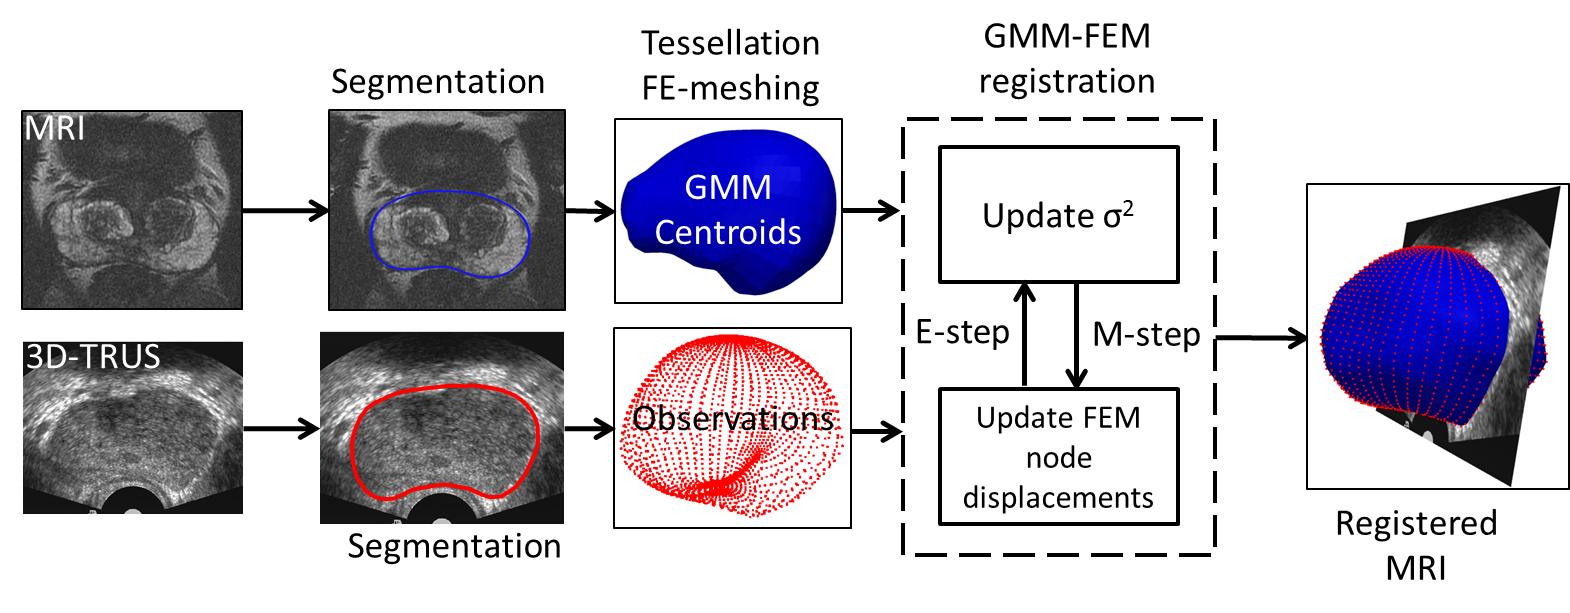
\includegraphics[width = 0.95\textwidth]{flow1}
\caption{Overview of the registration framework. The pre-operative (MR) image is taken before the procedure and is segmented to create a surface representation of the anatomy, in this case the prostate. This surface is then used to create an FE model of the volume. At the beginning of the procedure, an intra-operative (3D-TRUS) image is acquired and parts of the anatomy (midgland) are segmented. The GMM-FEM registration maps targets from the surface in the pre-operative plan to that of the intra-operative space.}
\label{fig:flowchart}
\end{figure*}
%%%%%%%%%%%%%%%%%%%%%%%%%%%%%%%%%%%%%%
An outline of our proposed GMM-FEM registration approach is shown in Figure~\ref{fig:flowchart}. We model the surface-to-surface registration as an expectation-maximization problem.  One surface is used to construct a probability density function for defining the boundary of the structure, and the other is considered a set of observations.  We wish to find the set of deformations that maximizes the likelihood that the observations came from the transformed probability distribution.

To define the probability distribution, we use a Gaussian-mixture model (GMM), which has been widely used to establish soft correspondences~\cite{Myronenko10a,Rasoulian12a,Jian11a}. A GMM is a parametric probability density function represented as a weighted sum of Gaussian densities.  Vertices of the source surface are assumed to be the centroids of Gaussian components, each represented by a mean and a variance. For simplicity, we take the variance to be isotropic in all directions for all components.  In this work, the source surface is extracted from the MRI and, the target surface (i.e. observations) are extracted from the TRUS.  A full list of notations is presented in Table \ref{tbl:notation}.
%%%%%%%%%%%%%%%%%%%%%%%%%%%%%%%%%%%%%%
\begin{table}[!bht]
  \centering
  \caption{Mathematical Notations \label{tbl:notation}}
  \begin{tabular}{lp{0.55\columnwidth}}
  \hline
    $D$ & Dimension of the surfaces\\
    $X_{N\times D}$ & Observations\\
    $Y_{M\times D}$ & GMM centroids\\
    $U_{J\times D}$ & FEM nodal displacements\\
    $x_n$ & n-th point of observations\\
    $y_m$ & m-th GMM centroids\\
    $\vec{x}_{DN \times 1},\vec{y}_{DM \times 1},\vec{u}_{DJ \times 1}$ & Rasterized representation of $X$, $Y$ and $U$\\
    $\Phi_{M\times J}$ & FEM interpolation matrix\\
    $K$ & Stiffness matrix\\
    $E$ & Young's modulus\\
    $\nu$ & Poisson's ratio\\
    $P_{M\times N}$ & GMM posterior probabilities\\ 
    $\sigma^2$ & Variance of Gaussian components\\
    $0{\leq}w{\leq}1$ & Estimate of outliers/missing data\\
    $\diag{(\vec{v})}$ & Diagonal matrix of a vector $\vec{v}$\\
    $I$ & Identity matrix\\
    $\tilde{P} = \kron{(P,I_{D\times{D}})}$ &Kronecker product of $P$ and $I$\\
    $1$ & Column vector of all ones\\
    \hline\\
  \end{tabular}
\end{table}
%%%%%%%%%%%%%%%%%%%%%%%%%%%%%%%%%\comment{What is the motivation for this?  I think we need to start from the beginning, with $y_m + v_m$, then say that since we are dealing with FE nodes but this expression only involves points on the surface of the model, we need an interpolation matrix $\Phi$.}
%%%%%%%%%%%%%%%%%%%%%%%%%%%%%%%%%%%%%%
\subsection{GMM-FEM Registration}
%%%%%%%%%%%%%%%%%%%%%%%%%%%%%%%%%%%%%%
The non-rigid registration is constrained by minimizing the volumetric strain energy of an FE model. Note that to form an FE model from a surface, we often need to add nodes interior to the surface. This can be done with most FE-meshing tools, such as TetGen \cite{Si06a}. In place of setting boundary conditions, we drive the surface of the model using implicit surface-to-surface forces, from source to target. These forces arise naturally by minimizing the log-likelihood function: 
%%%%%%%%%%%%%%%%%%%%%%%%%%%%%%%%%\Phi_mU
\begin{equation} \label{eq:loglike}
E(U,\sigma^2) = -\sum_{n=1}^N\log\sum_{m=1}^MP(y_m)P(x_n|y_m+v_m),
\end{equation}
%%%%%%%%%%%%%%%%%%%%%%%%%%%%%%%%%
where $v_m$ represents the nonrigid deformation field at the m-th GMM centroid. Since this expression only involves points on the surface of the model, we use an interpolation matrix $v_m={\Phi_m}U$ to relate surface displacements to nodal displacements. In our implementation, all points on the surface correspond to FE nodes, and internal nodes are appended to the end of the node list. As a result, the interpolation matrix has the form, $\Phi=\begin{bmatrix} I_{M\times M} & 0\\ 0 & 0 \end{bmatrix}$.   Subsequently, the unknowns, i.e. $\sigma^2$ and $U$, are solved using an Expectation Maximization (EM) algorithm. Initially, the variance is estimated as Myronenko~\textit{et~al.}~\cite{Myronenko10a}
%%%%%%%%%%%%%%%%%%%%%%%%%%%%%%%%%
\begin{equation} \label{eq:initVariance}
\sigma^2 = \frac{1}{DNM}\sum_{n=1}^{N}\sum_{m=1}^{M}\left\|x_n-y_m\right\|^2.
\end{equation}
%%%%%%%%%%%%%%%%%%%%%%%%%%%%%%%%%
In the expectation step, we compute how likely an observation corresponds to a GMM centroid by calculating the posterior probability
%%%%%%%%%%%%%%%%%%%%%%%%%%%%%%%%%
\begin{equation} \label{eq:prob}
P(x_n|y_m+\phi_mU) = \frac{\exp{\left(-\frac{1}{2}\frac{\left\|x_n -(y_m+\Phi_mU)\right\|^2}{\sigma^2}\right)}}{\sum_{j=1}^M\exp{\left(-\frac{1}{2}\frac{\left\|x_n -(y_j+\Phi_jU)\right\|^2}{\sigma^2}\right)} + c},
\end{equation}
%%%%%%%%%%%%%%%%%%%%%%%%%%%%%%%%%
where $c=(2\pi\sigma^2)^{D/2}\frac{w}{1-w}\frac{M}{N}$ is the contribution of an additional uniform distribution to account for noise, outliers and missing data. $0{\leq}w{\leq}1$ controls the weight of equal membership probabilities, set to zero if observations do not exhibit any noise, outliers or missing data. A value of one denotes that no correspondence between observations and GMM centroids can be made. Ignoring constants independent of $U,\sigma^2$, we can rewrite the maximization step of Equation~\eqref{eq:loglike} with an added FE regularizer:
%%%%%%%%%%%%%%%%%%%%%%%%%%%%%%%%%
\begin{eqnarray} \label{eq:obj}
Q(U,\sigma^2) &=& \frac{1}{2\sigma^2}\sum_{m,n=1}^{M,N}P(y_m|x_n)\left\|x_n- (y_m+\Phi_mU)\right\|^2 \nonumber\\
&& + \frac{N_PD}{2}\log(\sigma^2) + \frac{\beta}{2}\trans{\vec{u}}K\vec{u},
\end{eqnarray}
%%%%%%%%%%%%%%%%%%%%%%%%%%%%%%%%%
where $N_P=\sum_{m,n=1}^{M,N}P(y_m|x_n)$. The $\beta$ parameter controls the trade-off between the tightness of the fit and regularization. The stiffness matrix $K$ is derived directly from the FE model assuming a linear material.  Full details of this computation are given in Appendix~\ref{ap:FEM}. 

To simplify the numerical implementation, we can rewrite Equation~\eqref{eq:obj} into a rasterized vector form:
%%%%%%%%%%%%%%%%%%%%%%%%%%%%%%%%%
\begin{align}\label{eq:matrixrep}
    Q(\vec{u},\sigma^2) & = \dfrac{1}{2\sigma^2}\left[ \trans{\vec{x}}\diag\left(\trans{\tilde{P}}1\right)\vec{x} -2\;\trans{\vec{x}}\trans{\tilde{P}}(\vec{y}+\tilde{\Phi}\vec{u}) \right.\notag\\
    & \qquad \left. +\;\trans{(\vec{y}+\tilde{\Phi}\vec{u})}\diag\left(\tilde{P}1\right)(\vec{y}+\tilde{\Phi}\vec{u}) \right]\notag\\
    & \qquad + \dfrac{N_PD}{2}\log(\sigma^2) + \dfrac{\beta}{2}\trans{\vec{u}}K\vec{u}.
\end{align}
%%%%%%%%%%%%%%%%%%%%%%%%%%%%%%%%%
Optimal nodal displacements are obtained by minimizing Equation~\eqref{eq:matrixrep} with respect to the vector $\vec{u}$. This yields the sparse linear system
%%%%%%%%%%%%%%%%%%%%%%%%%%%%%%%%%
\begin{align}\label{eq:Mstep}
        \left[\trans{\tilde{\Phi}}\diag\!\left(\tilde{P}1\right)\tilde{\Phi} 
            + \beta \sigma^2K\right] \vec{u} & = \left[\trans{\tilde{\Phi}}\tilde{P}\vec{x}
            -\trans{\tilde{\Phi}}\diag\!\left(\tilde{P}1\right)\vec{y}\right],
\end{align}
%%%%%%%%%%%%%%%%%%%%%%%%%%%%%%%%%
which can easily be solved for the nodal displacements $\vec{u}$ using any sparse linear solver.  Now that we have an updated estimate of FE nodal displacements (and hence locations), we update the GMM probability distribution.  

The algorithm iterates between the expectation step (updating $\sigma^2$) and maximization step (updating $\vec{u}$) until the variance drops below a certain threshold.  The expectation step is exactly as in Myronenko~\textit{et~al.}~\cite{Myronenko10a} and is presented here only for completeness:
%%%%%%%%%%%%%%%%%%%%%%%%%%%%%%%%%
\begin{align}
\sigma^2 = & \frac{1}{N_PD}\sum_{m,n=1}^{M,N}\left\|x_n- (y_m+\Phi_mU)\right\|^2 \nonumber\\
= & \frac{1}{N_PD}\left[\trace\!\left(X^T\diag(P^T1)X\right)-2\trace\!\left((PX)^T(Y+{\Phi}U)\right)\right.\nonumber\\
& \left.+\trace\!\left((Y+{\Phi}U)^T\diag(P1)(Y+{\Phi}U)\right)\right], \label{eq:estep1}
\end{align}
%%%%%%%%%%%%%%%%%%%%%%%%%%%%%%%%%
which is equivalent to the following in rasterized representation:
%%%%%%%%%%%%%%%%%%%%%%%%%%%%%%%%%
\begin{align} 
\sigma^2 = & \frac{1}{N_PD}\left[\vec{x}^t\diag\!\left(\tilde{P}^T1\right)\vec{x} -2\vec{x}^T\tilde{P}^T(\vec{y}+\tilde{\Phi}\vec{u})\right.\nonumber\\
  & \left.+(\vec{y}+\tilde{\Phi}\vec{u})^T\diag\!\left(\tilde{P}1\right)(\vec{y}+\tilde{\Phi}\vec{u})\right]. \label{eq:estep2}
\end{align}
%%%%%%%%%%%%%%%%%%%%%%%%%%%%%%%%%
For biomechanical material properties, we apply a homogeneous elastic material with a constant Young's modulus to all elements. To segment the prostatectomy and biopsy data, we used Stradwin~\cite{Treece00a} and 3D Slicer~\cite{Fedorov12a}, respectively. We then used TetGen~\cite{Si06a} to create a tetrahedral volumetric mesh of the prostate.  The models used in this study are composed of $\approx7500$ elements. Throughout our experiments, we used a stopping condition of $\sigma^2\leq1e^{-4}~\mathrm{mm}^2$, Young's modulus of $E=5$~kPa, which is in the range of values reported in~\cite{Kemper04a} for the prostate, and a Poisson's ratio of $\nu=0.49$. We investigate the sensitivity to biomechanical properties in Section~\ref{sec:exp3}.

%%%%%%%%%%%%%%%%%%%%%%%%%%%%%%%%%
\subsection{Relationship to CPD}
%%%%%%%%%%%%%%%%%%%%%%%%%%%%%%%%%
The proposed registration algorithm builds on the soft correspondence approach proposed by Myronenko~\textit{et~al.}~\cite{Myronenko10a}. In the original CPD algorithm, the maximization step solves for the optimal set of weights, $W$, that satisfies
%%%%%%%%%%%%%%%%%%%%%%%%%%%%%%%%%
\begin{equation} \label{eq:cpd1}
\left[\diag(P1)G + \lambda\sigma^2I\right]W = PX - \diag\left(P1\right)Y,
\end{equation}
%%%%%%%%%%%%%%%%%%%%%%%%%%%%%%%%%
where $G_{M \times M}$ is a kernel matrix with elements $g_{ij}=\exp{\left(-\frac{\left\|y_i- y_j)\right\|^2}{2\beta^2}\right)}$ and $\beta$ is the width of the Gaussian which controls motion coherence of the model (i.e.~coherence width). Writing Equation~\eqref{eq:cpd1} in rasterized form yields
%%%%%%%%%%%%%%%%%%%%%%%%%%%%%%%%%
\begin{equation} \label{eq:cpd2}
\left[\diag(\tilde{P}1)\tilde{G} + \lambda\sigma^2\tilde{I}\right]\vec{w} = [\tilde{P}\vec{x} - \diag\left(\tilde{P}1\right)\vec{y}].
\end{equation}
%%%%%%%%%%%%%%%%%%%%%%%%%%%%%%%%%
While CPD registration has been shown to be an effective tool for registering surfaces, the internal deformation field is not directly regularized. Instead, coherence of the surface is enforced by applying a low-pass filter on surface deformation modes.  To create a deformation map for the entire volume, interior displacements need to be interpolated based on those at the surface.  Instead of this two-step process, we use a physics-inspired FE model to simultaneously regularize and provide a full volumetric deformation map.
%%%%%%%%%%%%%%%%%%%%%%%%%%%%%%%%%
\subsection{Related Registration Methods Used for Comparison}
%%%%%%%%%%%%%%%%%%%%%%%%%%%%%%%%%
This section provides a minimal description of the two registration methods that have been used as a basis for comparison. For a detailed discussion on the mechanics of these methods, the reader is referred to relevant papers~\cite{Chui03a,Ferrant01a}.
%%%%%%%%%%%%%%%%%%%%%%%%%%%%%%%%%
\subsubsection{TPS-RPM}\label{sec:tpsrpm}
%%%%%%%%%%%%%%%%%%%%%%%%%%%%%%%%%
This algorithm solves the registration problem using a similar EM algorithm. The authors use deterministic annealing in the expectation step to decrease both the temperature, $T$, and the regularization weights, $\{\lambda_1, \lambda_2\}$ i.e. Equations (3) and (8) in~\cite{Chui03a}. The temperature in their framework corresponds to variance in ours. The maximization step, Equation (19) in~\cite{Chui03a}, can be written as
%%%%%%%%%%%%%%%%%%%%%%%%%%%%%%%%%
\begin{align}
\argmin_{(d,w)} E(d,w) = & \argmin_{(d,w)} \left\|MX-Yd-{\Psi}w\right\|^2 \nonumber\\
  & + {\lambda_1}\trace({\trans{w}{\Psi}w})\nonumber\\
  & + {\lambda_2}\trace({\trans{(d-I)}(d-I)}), \label{eq:tpsrpm}
\end{align}
%%%%%%%%%%%%%%%%%%%%%%%%%%%%%%%%%
where $M$ is the correspondence matrix, $\Psi$ is the 3D TPS kernel, $w$ are the TPS weights, $d$ is the affine component of the total transform and $\lambda_1$ and $\lambda_2$ control the contribution of affine and nonrigid components. We use the open-source Matlab version of TPS-RPM that is freely available to the scientific community\footnote{\url{http://noodle.med.yale.edu/~chui/tps-rpm.html}}. Following the registration, in order to calculate the internal deformation field, we used the TPS kernel to propagate surface deformations inside the prostate as described in~\cite{Sibson91a}.
%%%%%%%%%%%%%%%%%%%%%%%%%%%%%%%%%
\subsubsection{ICP-FEM}\label{sec:icpfem}
%%%%%%%%%%%%%%%%%%%%%%%%%%%%%%%%%
The FE-based registration approach by Ferrant~\textit{et~al.}~\cite{Ferrant01a} deforms the surface of the source object to that of the target using image-driven forces. The system evolves through time by iteratively applying external forces to the surface of the membrane. Deformations of the surface are discretized using finite differences which yields a semi-implicit update method for nodal displacements:
%%%%%%%%%%%%%%%%%%%%%%%%%%%%%%%%%
\begin{equation}\label{eq:icpfem}
(I+\tau{K})u^t = u^{t-1} - \tau{F^t},
\end{equation}
%%%%%%%%%%%%%%%%%%%%%%%%%%%%%%%%%
where $\tau$ is the time step, $F^t$ is the current estimate of surface forces, $u^{t-1}$ are the previous nodal displacements and $u^t$ is the next estimate of nodal displacements. Image forces are determined by a local search, driving the surface nodes of the FE-model to the nearest sharp feature in the image.  In our surface-based registration, instead of using image forces, we use ICP to estimate the nearest features, which are then used to apply surface forces. This is the point-cloud analogue of Ferrant~\textit{et~al.}~\cite{Ferrant01a}.
%%%%%%%%%%%%%%%%%%%%%%%%%%%%%%%%%
\section{Experiments and Results}
%%%%%%%%%%%%%%%%%%%%%%%%%%%%%%%%%
In this section, we evaluate the proposed nonrigid registration method in a series of experiments with MR-TRUS image pairs acquired from patients who underwent a prostate intervention. The data acquisition protocol was approved by the institutional ethics board, and in each case patients provided written consent to be included in the study. The rest of this section is divided into three subsections. In Section~\ref{sec:data}, we discuss the data acquisition, segmentation protocol and the initialization of the registration. Subsequently, we validate our registration method using intrinsic fiducials found in the interior of the prostate, and compare to two other surface-based registration methods (i.e. TPS-RPM and ICP-FEM). Accuracy is quantitatively evaluated by measuring the TRE between pairs of fiducials found interior to the prostate. This is described in Section~\ref{sec:exp1}. To test the importance of including the FE regularizer in-loop, in Section~\ref{sec:exp2}, we compare to a method in which the final deformation field is only computed as a post-processing step. Finally, in Section~\ref{sec:exp3}, we investigate the sensitivity of our approach to biomechanical parameters that control the regularization term in the registration.
%%%%%%%%%%%%%%%%%%%%%%%%%%%%%%%%%
\subsection{Data}\label{sec:data}
%%%%%%%%%%%%%%%%%%%%%%%%%%%%%%%%%
\begin{figure}[t]
	\centering
	\subfloat[][Ex~vivo prostate\label{fig:prostdata1}]{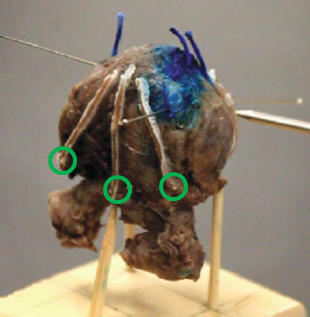
\includegraphics[width=0.3\columnwidth,height=1.2in]{prostatectomydata1}}
	\subfloat[][Ex~vivo MRI\label{fig:prostdata2}]{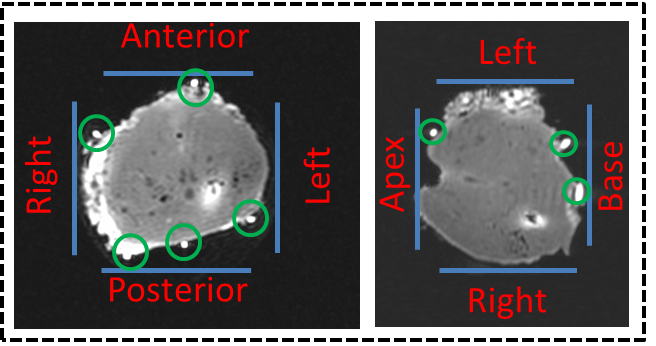
\includegraphics[width=0.60\columnwidth,height=1.2in]{prostatectomydata2}}\\
	\subfloat[][Initial alignment\label{fig:prostdata4}]{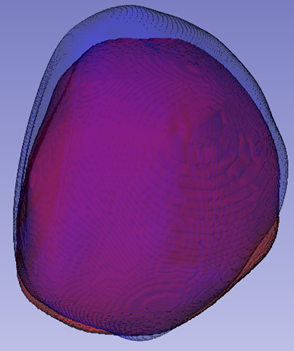
\includegraphics[width=0.3\columnwidth,height=1.2in]{US_initial_prostatectomy}}
	\subfloat[][In~vivo TRUS\label{fig:prostdata3}]{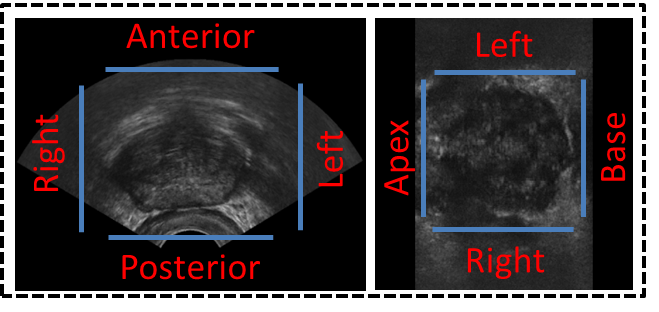
\includegraphics[width=0.60\columnwidth,height=1.2in]{prostatectomydata3}}
\caption{Prostatectomy data collection protocol. Following the prostatectomy, strand-shaped fiducials are attached to the prostate to mark anatomical coordinates of the prostate in the MR. These strands are highlighted with a green circle on the prostate (a) and are visible MRI (b). During the prostatectomy, a volumetric US is acquired using a side-firing probe (d). Both MR and TRUS images are segmented and brought to an initial alignment at the beginning of the registration (c). \label{fig:prostatectomyData}}
\end{figure}
%%%%%%%%%%%%%%%%%%%%%%%%%%%%%%%%%
\subsubsection{Prostatectomy}\label{sec:data1}
%%%%%%%%%%%%%%%%%%%%%%%%%%%%%%%%%
We acquired MR and TRUS volumes of ten patients scheduled for a prostatectomy. Due to nonrigid deformations induced during the fixation process, the changes in shape of the prostate cannot be captured using a rigid or affine transformation alone. Figure~\ref{fig:prostatectomyData} shows the major steps in the data acquisition and alignment protocol. The TRUS volumes were collected with an Ultrasonix Touch machine (Ultrasonix, Richmond, Canada) using a BPL-95/55 side firing transducer mounted on a motorized cradle. The parasagittal 2D-TRUS images were acquired at $5^\circ$ intervals and reconstructed into a 3D-TRUS volume with an axial and lateral spacings of $0.12$~mm. This is shown in Figure~\ref{fig:prostdata3}. Following the prostatectomy, the prostate was fixated in a $10\%$ buffered formalin solution for perservation and MR-visible strand-shaped fiducial markers were applied to the specimen using the protocol by Gibson~\textit{et~al.}~\cite{Gibson12a}. This is shown in Figure~\ref{fig:prostdata1}. Specimens were scanned using a Discovery MR750 scanner (GE Healthcare, Waukesha, USA) at 3T using an endorectal coil (Prostate eCoil, Medrad, Warrendale, USA) to acquire T1-weighted MR images with a $0.3$~mm slice thickness. This is shown in Figure~\ref{fig:prostdata2}. Both the MR and TRUS volumes were manually segmented under the supervision of an expert clinican. Finally, as seen in Figure~\ref{fig:prostdata3}, the two segmentations were brought into a manual initial alignment using the orientation information from the strands and rough anatomical locations of the based and apex.
%%%%%%%%%%%%%%%%%%%%%%%%%%%%%%%%%
\begin{figure}[t]
	\centering
	\subfloat[][Segmented MRI (blue)\label{fig:biopsy1}]{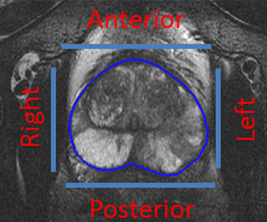
\includegraphics[width=0.3\columnwidth,height=1.0in]{ProstateBiopsy_MR}} \hfill
	\subfloat[][Segmented TRUS (red)\label{fig:biopsy2}]{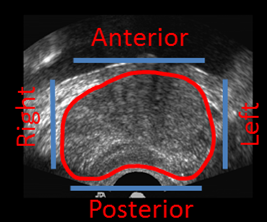
\includegraphics[width=0.3\columnwidth,height=1.0in]{ProstateBiopsy_US}} \hfill
	\subfloat[][Initialization of the MRI (blue) and TRUS (red)\label{fig:biopsy3}]{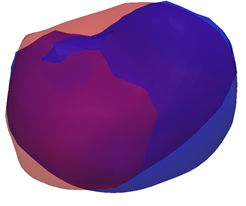
\includegraphics[width=0.3\columnwidth,height=1.0in]{ProstateBiopsy_Initial}}
  \caption{An axial slice of the T2-weighted MRI (a). An axial slice 3D-TRUS volume (b). The segmented MRI (blue) and 3D-TRUS (red) are initialized using RAS axis and center of mass alignment (c). \label{fig:biopsy}}
\end{figure}
%%%%%%%%%%%%%%%%%%%%%%%%%%%%%%%%%
\subsubsection{Prostate Biopsy}\label{sec:data2}
The second set of data was acquired from ten patients scheduled for prostate biopsy. Figure~\ref{fig:biopsy} shows the major steps of our data collection, segmentation and initialization protocol. We acquired T2-weighted MR images from ten patients using a 3 Tesla GE Excite HD MRI system (Milwaukee, WI, USA) with a spacing of $0.27~\times~0.27~\times~2.2$ mm. This step is shown in Figure~\ref{fig:biopsy1}. The TRUS images were acquired using a 3D-TRUS mechanical biopsy system~\cite{Bax08a} with a Philips HDI-5000 US machine and a C9-5 transducer using an axial rotation of the biopsy probe. The TRUS images were reconstructed into a 3D-volume with a spacing of $0.19~\times~0.19~\times~0.19$ mm. These images were segmented under the supervision of an expert urologist. This step is shown in Figure~\ref{fig:biopsy2}. Finally, as shown in Figure~\ref{fig:biopsy3}, the prostate surfaces from the MRI and TRUS were brought to an initial position using right-anterior-superior (RAS) coordinates and center of mass alignment.
%%%%%%%%%%%%%%%%%%%%%%%%%%%%%%%%%
\subsubsection{Global Registration}\label{sec:data3}
%%%%%%%%%%%%%%%%%%%%%%%%%%%%%%%%%
Following initial alignment, we performed a global registration using CPD~\cite{Myronenko10a} between MR and TRUS surfaces to compensate for residual errors in the position and orientation. For the prostatectomy data, we opted to perform an affine registration to compensate for the bulk of non-linearities due to the ex~vivo nature of the data. The global registration has only one free parameter, $w$, set to zero for prostatectomy surfaces that do not have missing data points. For prostate biopsy surfaces, data was collected in vivo, so we expect that any changes in shape have a mostly biomechanical nature.  For this reason, we initialize the registration with a simple rigid alignment.  The US images from the biopsies are not as clear as those from the prostatectomy, so we estimate the number of outliers caused by errors in segmentation to $w=0.1$.

% \note{Reasons for Affine vs Rigid: The changes in the shape of the ex vivo data are not purely mechanical, however, we can still use the small deformation model of FEMs, provided that the large deformations due to formalin fixation are removed. The prostate biopsy data is collected in vivo. As a result, changes in shape should be mostly mechanical.}
%%%%%%%%%%%%%%%%%%%%%%%%%%%%%%%%%
\subsection{Registration to Full and Partial Surfaces}\label{sec:exp1}
%%%%%%%%%%%%%%%%%%%%%%%%%%%%%%%%%
\subsubsection{Prostatectomy}
%%%%%%%%%%%%%%%%%%%%%%%%%%%%%%%%%
As a first set of experiments, we used the prostatectomy data described in Section~\ref{sec:data1} to validate our registration pipeline. Figure~\ref{fig:exp2reg1} shows a typical affine registration result which is the starting point for our nonrigid registration. Figures~\ref{fig:exp1reg2}, \ref{fig:exp1reg3} and \ref{fig:exp1reg4} show the result of TPS-RPM, ICP-FEM and our proposed GMM-FEM registration, respectively. For our GMM-FEM method, we set the estimate of outliers, $w$, to zero.
%%%%%%%%%%%%%%%%%%%%%%%%%%%%%%%%%
\begin{figure*}
	\centering
	\subfloat[][Affine, $\mathrm{Dice}=0.89$\label{fig:exp2reg1}]{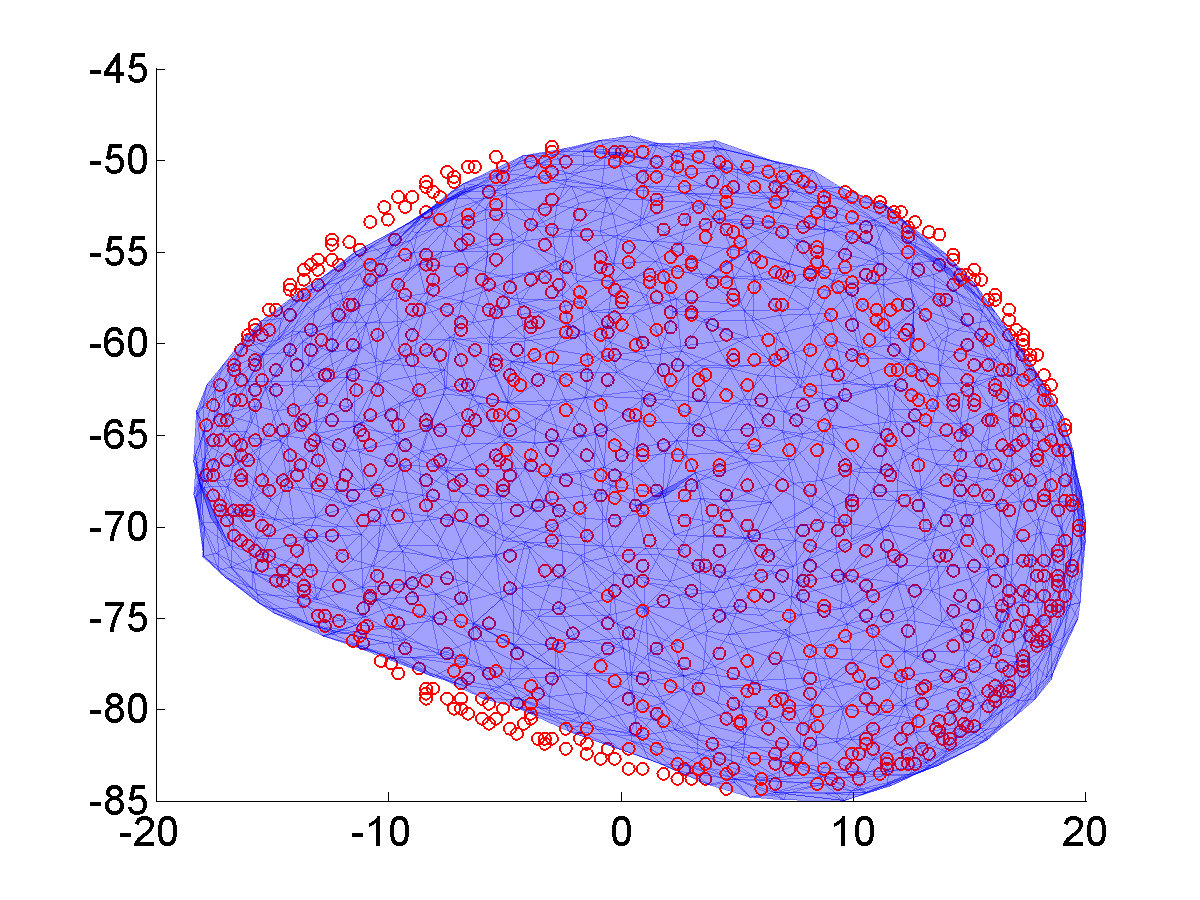
\includegraphics[width=0.45\textwidth]{P030_Affine}} \hfill
	\subfloat[][TPS-RPM with $T_i=10$ and $\lambda_1/{\lambda_2=0.01}$, $\mathrm{Dice}=1.00$\label{fig:exp2reg2}]{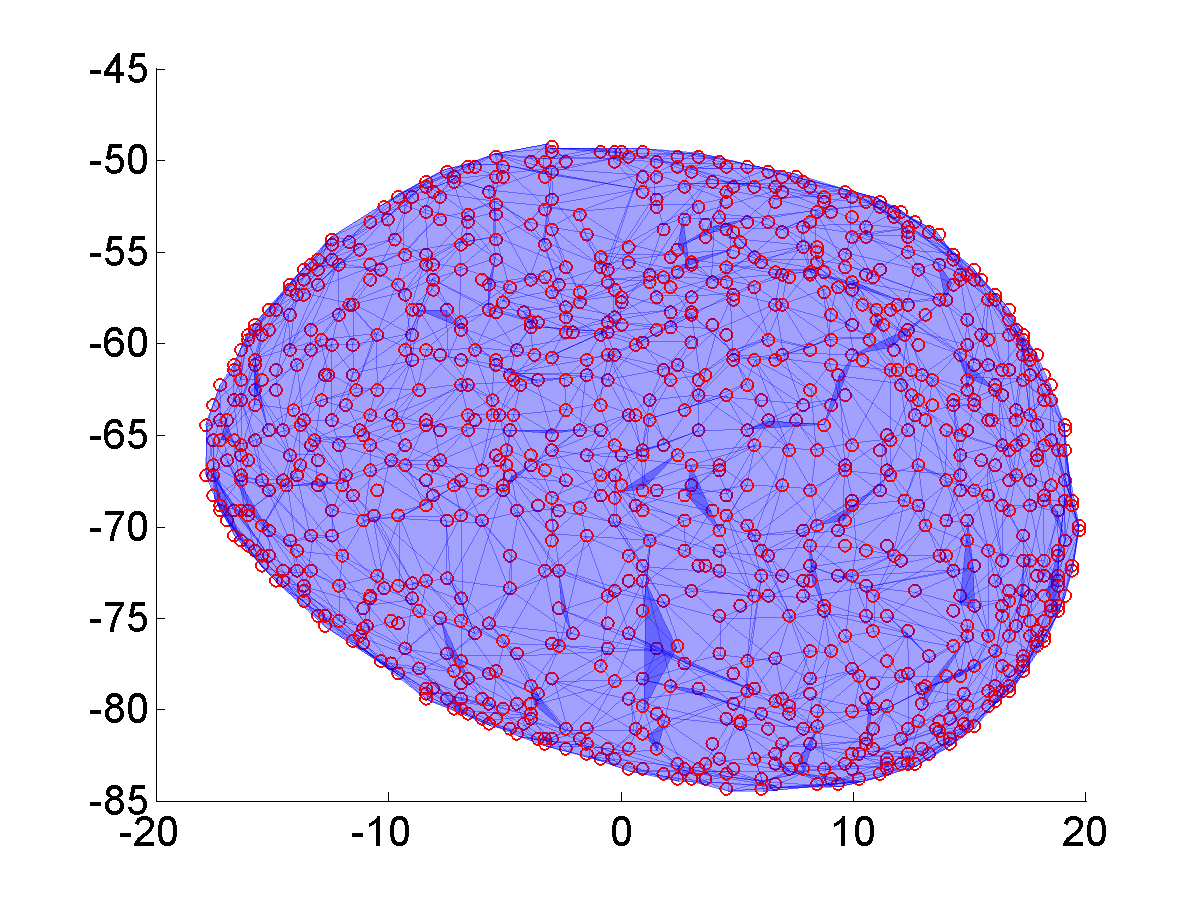
\includegraphics[width=0.45\textwidth]{P030_TPS_RPM}}\\
	\subfloat[][ICP-FEM with $\tau=0.1$, $E=0.1$~kPa and $\nu=0.49$, $\mathrm{Dice}=0.97$\label{fig:exp2reg3}]{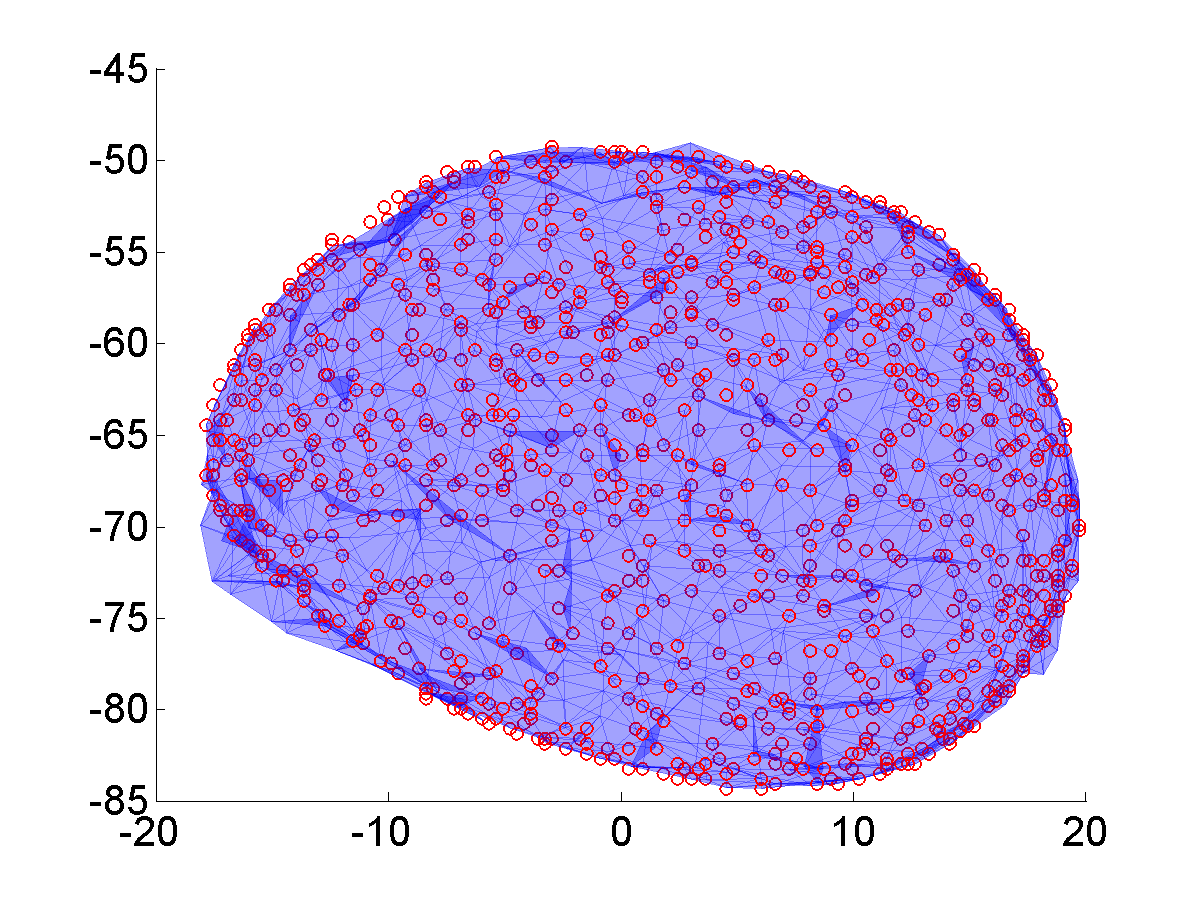
\includegraphics[width=0.45\textwidth]{P030_ICP_FEM}}\hfill
	\subfloat[][GMM-FEM with $E=5.0$~kPa, $\nu=0.49$ and $\beta=0.05$, $\mathrm{Dice}=0.99$\label{fig:exp2reg4}]{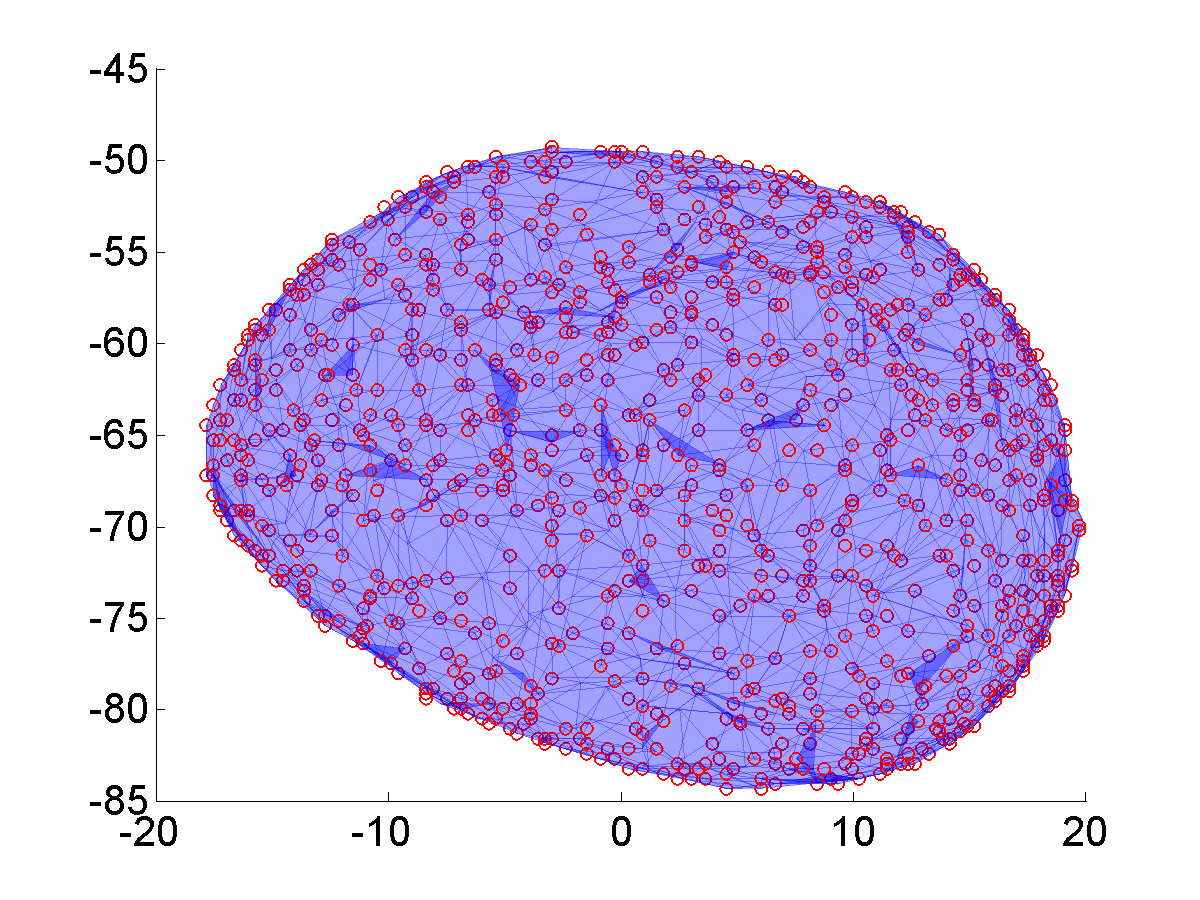
\includegraphics[width=0.45\textwidth]{P030_GMM_FEM}}
    \caption{An example of registration to full data. Registration results on prostatectomy data following surface based registration between the MR (blue) and TRUS (red) for: Rigid (a), TPS-RPM (b), ICP-FEM (c) and GMM-FEM (d). The estimate for missing data, $w$, was fixed at zero for all three nonrigid methods. \label{fig:exp2fig1}}
\end{figure*}
%%%%%%%%%%%%%%%%%%%%%%%%%%%%%%%%%
Throughout the experiment, for the two registration methods used for comparison, i.e. TPS-RPM and ICP-FEM, we tuned the parameters such that the best surface overlap and the best TRE was achieved. For TPS-RPM, the initial temperature was set to $T_i=10~\mathrm{mm}^2$ and the stopping condition was set to $T\leq0.2$~$\mathrm{mm}^2$. For ICP-FEM, the time step was set to $\tau=0.1$. Also, Young's modulus and Poisson's ratio were set to $E=0.1$~kPa and $\nu=0.49$, respectively. As seen in Figure~\ref{fig:exp2fig1}, all three nonrigid registration methods achieve a better surface overlap compared to affine registration alone. The improvement in the Dice similarity coefficient following nonrigid registration shows that these methods have converged.

In order to visualize the result of our GMM-FEM registration in the interior of the prostate, as shown in Figure~\ref{fig:exp2fig2}, we also resampled the MR image into the space of the TRUS. Figure~\ref{fig:exp2US} shows an axial slice of the prostate in the TRUS and corresponding GMM-FEM registered MRI, respectively. The magnitude of the deformation field at the same plane is shown in Figure~\ref{fig:exp2def}. Figure~\ref{fig:exp2ch} is the checkerboard comparison of Figure~\ref{fig:exp2gmmfem} and \ref{fig:exp2US}. As seen in Figure~\ref{fig:exp2ch}, the boundary of the prostate matches that of the TRUS, which is expected since the proposed method optimizes for best surface overlap. Also as seen in Figure~\ref{fig:exp2def}, the majority of the correction is made at regions near the boundary of the prostate, which is where surface-based forces are applied to the FE model.
%%%%%%%%%%%%%%%%%%%%%%%%%%%%%%%%%
\begin{figure}
	\centering
	\subfloat[][TRUS\label{fig:exp2US}]{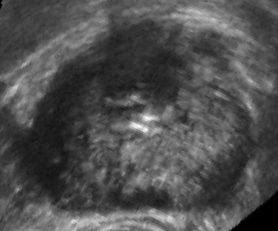
\includegraphics[width=0.45\columnwidth]{ProstatectomyResults_US}}\hfill
	\subfloat[][GMM-FEM\label{fig:exp2gmmfem}]{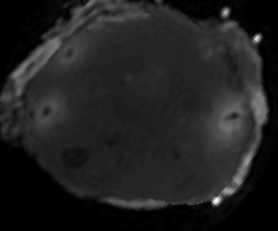
\includegraphics[width=0.45\columnwidth]{ProstatectomyResults_MR_FEM}}\\
	\subfloat[][Magnitude of the deformation field (mm)\label{fig:exp2def}]{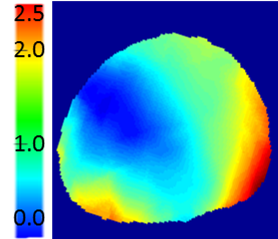
\includegraphics[width=0.45\columnwidth]{DeformationGridProstatectomy2}}\hfill
	\subfloat[][Comparison of (a) and (b)\label{fig:exp2ch}]{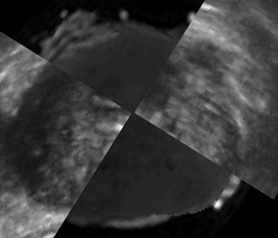
\includegraphics[width=0.45\columnwidth]{ProstatectomyResults_CH}}
   \caption{Typical results for a prostatectomy data. The axial slice of TRUS (a) and the corresponding GMM-FEM (b) registration results. The deformation map of the nonrigid registration and the corresponding TRUS slice (dashed line) are also shown in (c). The checkerboard of (a) and (b) is shown for comparison. \label{fig:exp2fig2}}
\end{figure}
%%%%%%%%%%%%%%%%%%%%%%%%%%%%%%%%%
\begin{figure}[t]
	\centering
	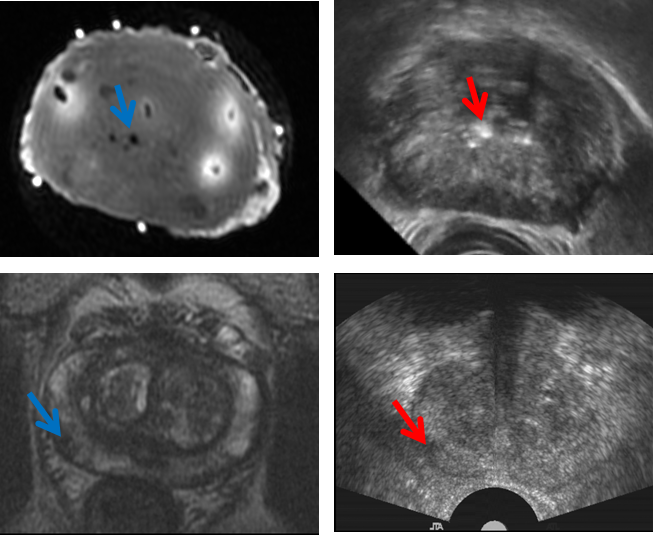
\includegraphics[width=\columnwidth]{FiducialPair}
	\caption{Examples of fiducial pairs in MR (left column) and TRUS (right column) for prostatectomy (top row) and biopsy (bottom row) data. \label{fig:exp2fiducial1}}
\end{figure}
%%%%%%%%%%%%%%%%%%%%%%%%%%%%%%%%%
\begin{table*}[tb]
\begin{center}
\caption{Mean and standard deviation of the TRE (mm) for prostatectomy data following affine and nonrigid registration.}
\centering
\begin{tabular}{c| c| c}
	\hline
	Method & TRE & $p$-value\\
	\hline
	Affine & $3.17 \pm 1.38$ & NA \\
	\hline
	TPS-RPM & $4.19 \pm 1.76$ & $6e-3$ \\
	\hline
	ICP-FEM & $3.00 \pm 1.39$ & $4e-7$ \\
	\hline
	GMM-FEM & $2.65 \pm 1.29$ & $1e-7$ \\
   \hline
\end{tabular}
\label{tab:exp2Res1}
\end{center}
\end{table*}
%%%%%%%%%%%%%%%%%%%%%%%%%%%%%%%%%
\begin{table*}[tb]
\begin{center}
\caption{Mean and standard deviation of the TRE (mm) for biopsy data following rigid and nonrigid registration.}
\centering
\begin{tabular}{c| c| c}
	\hline
	Method & TRE & $p$-value\\
	\hline
	Rigid & $4.44 \pm 1.51$ & NA \\
	\hline
	TPS-RPM & $7.2 \pm 2.31$ & $1e-7$ \\
	\hline
	ICP-FEM & $3.51 \pm 1.43$ & $4e-7$ \\
	\hline
	GMM-FEM & $2.64 \pm 1.1$ & $3e-7$ \\
   \hline
\end{tabular}
\label{tab:exp1Res1}
\end{center}
\end{table*}%%%%%%%%%%%%%%%%%%%%%%%%%%%%%%%%%
\subsubsection{Prostate Biopsy}
%%%%%%%%%%%%%%%%%%%%%%%%%%%%%%%%%
To further validate our registration results, we used the biopsy data which was described in Section~\ref{sec:data2}. In order to maintain the clinical requirements throughout our experiments, we segmented the prostate fully in the MR and only partially in TRUS, i.e. only eleven slices with a thickness of $2.0$~mm were segmented around the midgland. This resulted in a partial segmentation of the prostate, which was approximately 70\% of the base-apex axis of the prostate. Figure~\ref{fig:exp1reg1} shows a typical rigid registration outcome which is the starting point for our nonrigid registration. Figures~\ref{fig:exp1reg2}, \ref{fig:exp1reg3} and \ref{fig:exp1reg4} show the result of TPS-RPM, ICP-FEM and our proposed GMM-FEM registration, respectively. We do not report the Dice similarity coefficient for partial registration since parts of the base and apex were not segmented.

We observed that for larger estimates of missing data, the GMM-FEM registration treats large deformations as outliers and, subsequently, does not compensate for them. For very small estimates of outliers, $w\approx0$, the registration strives to overfit the FEM to the missing data. In our experiments, this resulted in unrealistic deformations, e.g. inverted elements, around the base and apex regions. Throughout the GMM-FEM registration, we set the estimate of outliers/missing data to $w=0.1$. For TPS-RPM, we followed the same outlier rejection in~\cite{Chui03a}, where points that cannot be reliably matched are assigned to a cluster with the initial temperature as its variance.

In order to visualize the result of our GMM-FEM registration in the interior of the prostate, as shown in Figure~\ref{fig:exp1fig2}, we resampled the MR image into the space of the TRUS for this dataset as well. Figures~\ref{fig:exp1US} and \ref{fig:exp1gmmfem} show an axial slice of the prostate in the TRUS and corresponding GMM-FEM slice, respectively. In Figure~\ref{fig:exp1ch} the checkerboard of TRUS and GMM-FEM registration of the two slices is shown for comparison. Also, the magnitude of the deformation field at this slice is shown in Figure~\ref{fig:exp1def}. Large corrections ($\approx2$~mm) are applied close to the rectum. This is to be expected, since the end-firing probe pushes against the prostate in this region.
%%%%%%%%%%%%%%%%%%%%%%%%%%%%%%%%%
\begin{figure*}
	\centering
	\subfloat[][Rigid\label{fig:exp1reg1}]{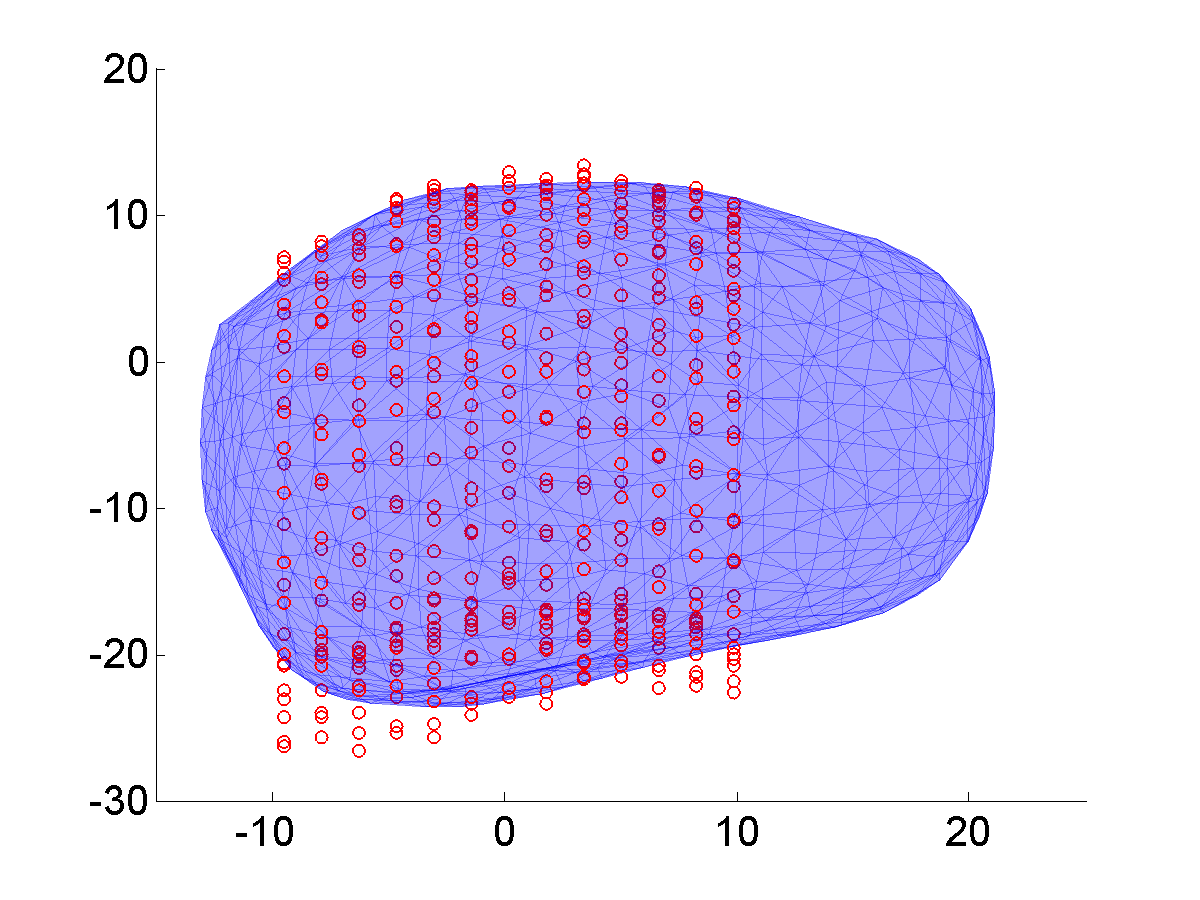
\includegraphics[width=0.45\textwidth]{P070_Rigid}}\hfill
	\subfloat[][TPS-RPM with $T_i=50$ and $\lambda_1/{\lambda_2=1e-5}$\label{fig:exp1reg2}]{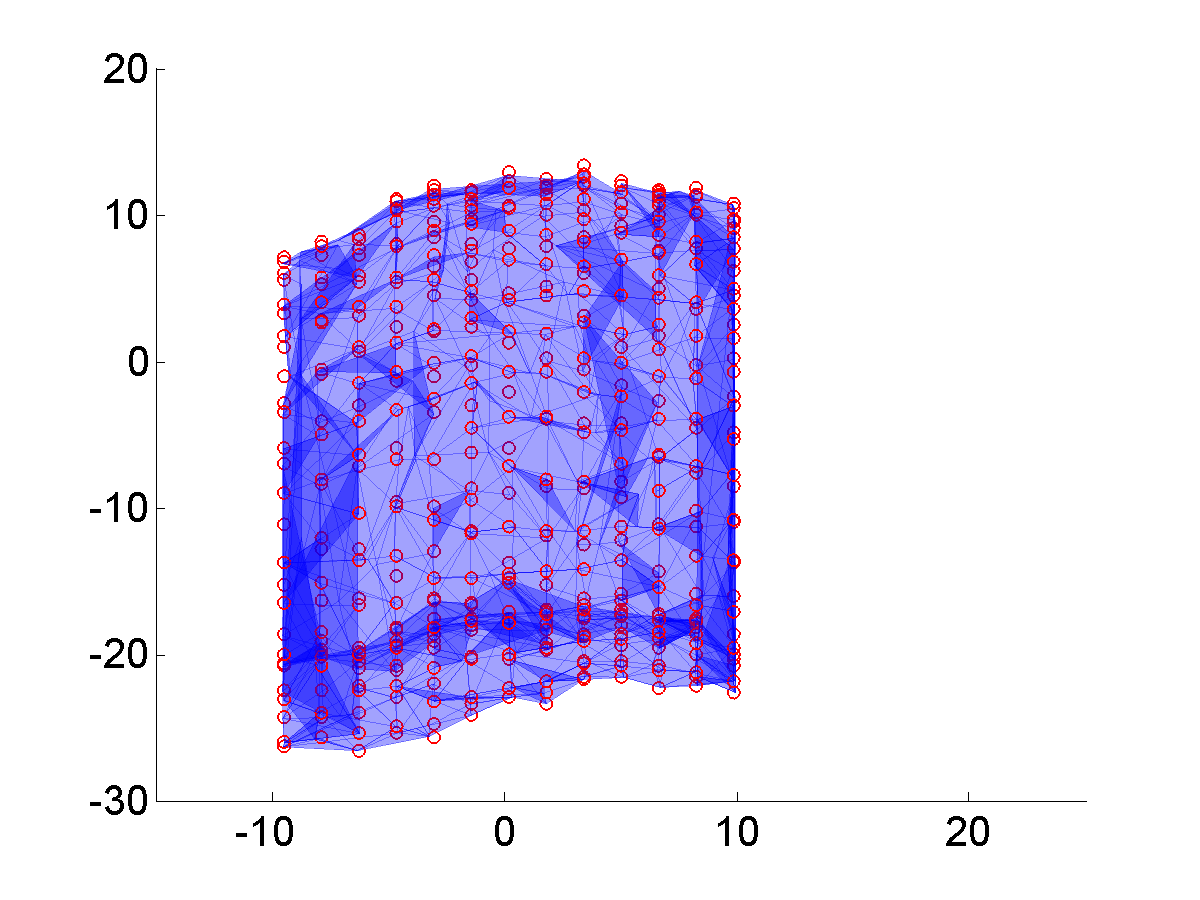
\includegraphics[width=0.45\textwidth]{P070_TPS_RPM}}\\
	\subfloat[][ICP-FEM with $\tau=0.1$, $E=0.1$~kPa and $\nu=0.49$\label{fig:exp1reg3}]{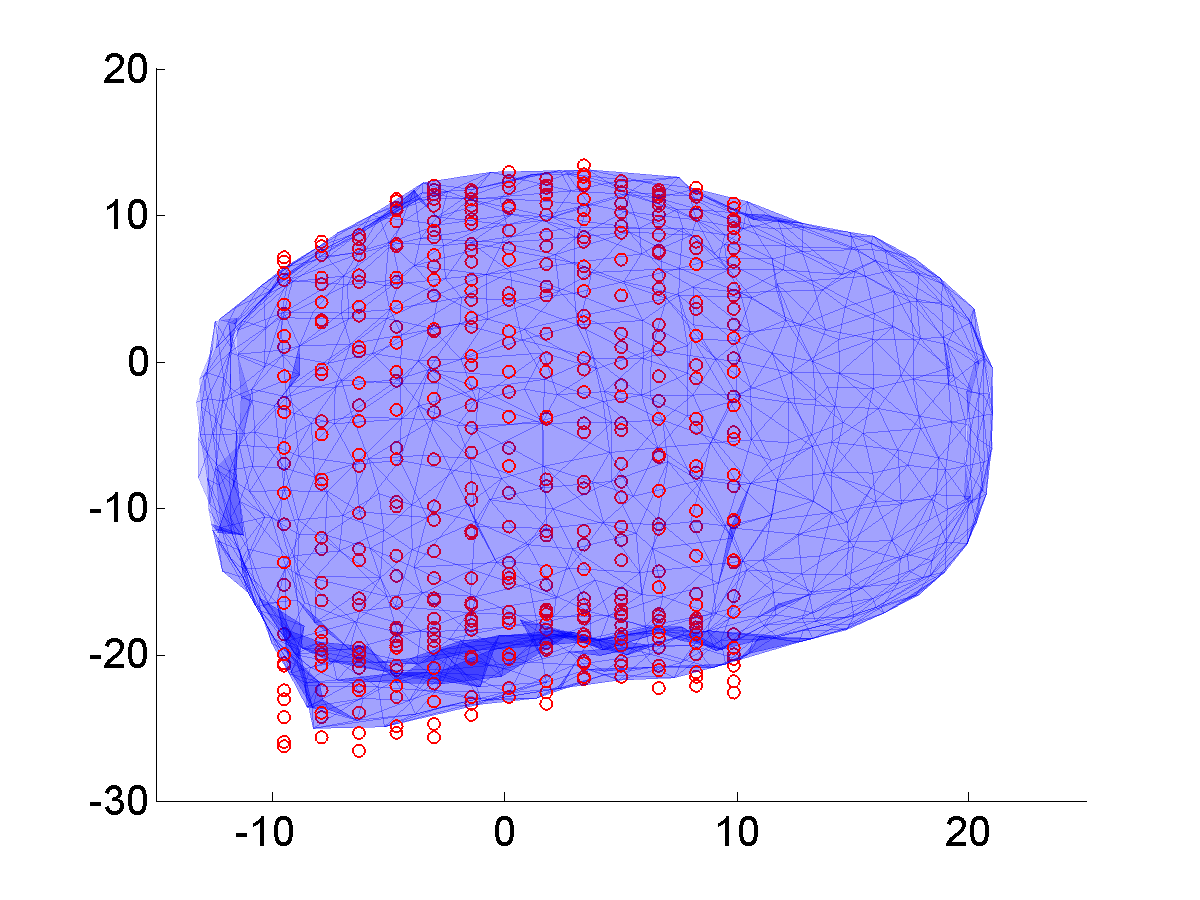
\includegraphics[width=0.45\textwidth]{P070_ICP_FEM}}\hfill
	% \subfloat[][GMM-FEM with $w=0.1$, $E=5.0$~kPa, $\nu=0.49$ and $\beta=0.05$\label{fig:exp1reg4}]{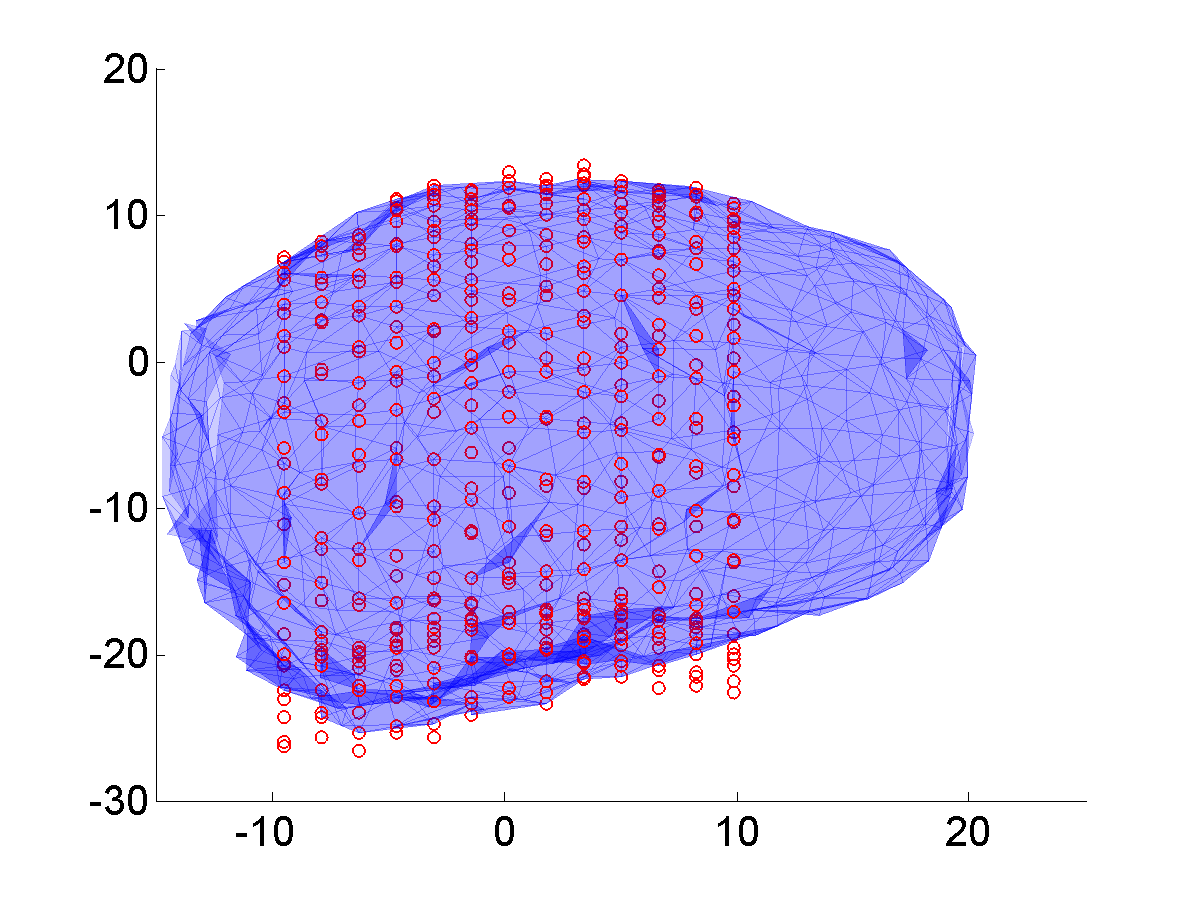
\includegraphics[width=0.45\textwidth]{P070_GMM_FEM}}
	\subfloat[][GMM-FEM with $w=0.1$, $E=5.0$~kPa, $\nu=0.49$ and $\beta=0.05$\label{fig:exp1reg4}]{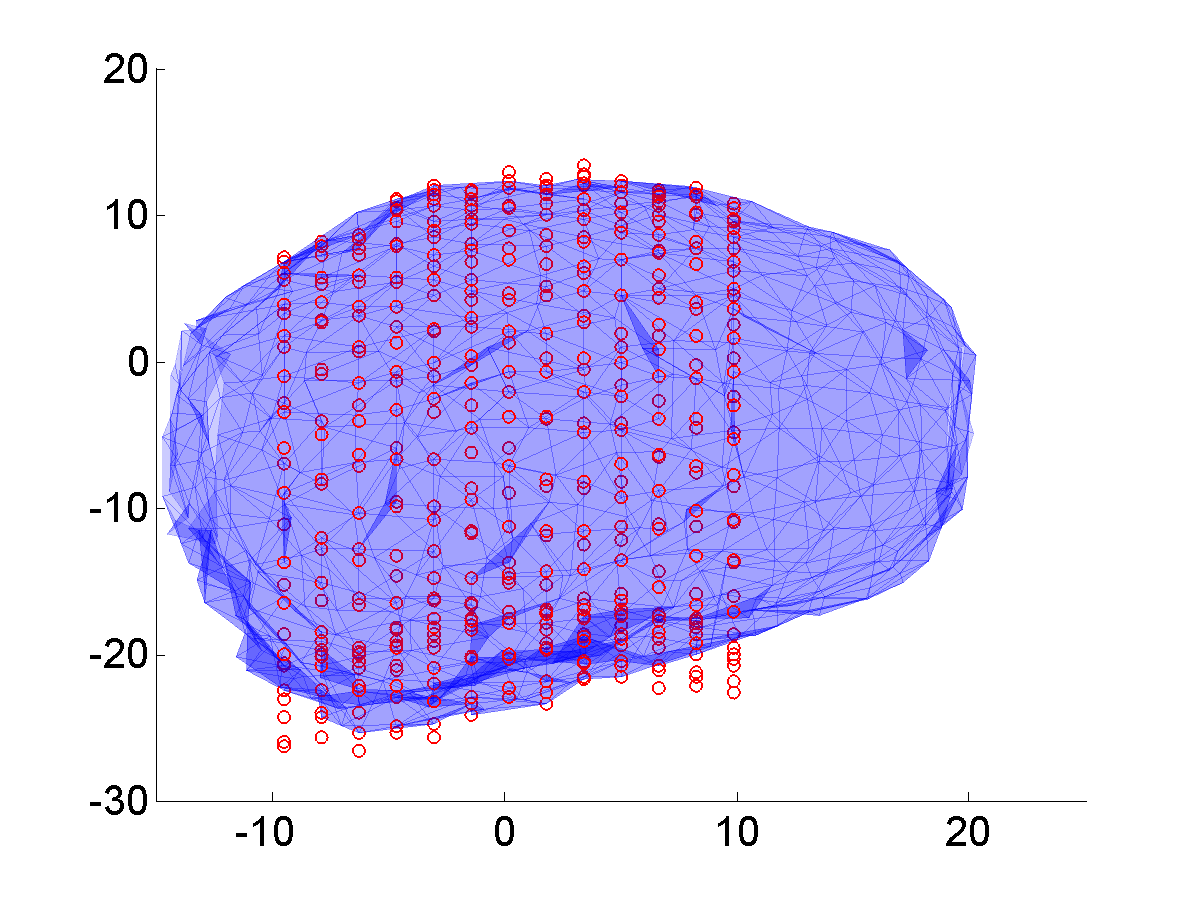
\includegraphics[width=0.45\textwidth]{P070_GMM_FEM}}
    \caption{An example of registration to missing data. Prostate biopsy results following surface based registration between the MR (blue) and TRUS (red) for: Rigid (a), TPS-RPM (b), ICP-FEM (c) and GMM-FEM (d). \label{fig:exp1fig1}}    
\end{figure*}
%%%%%%%%%%%%%%%%%%%%%%%%%%%%%%%%%
\begin{figure}
	\centering
	\subfloat[][TRUS\label{fig:exp1US}]{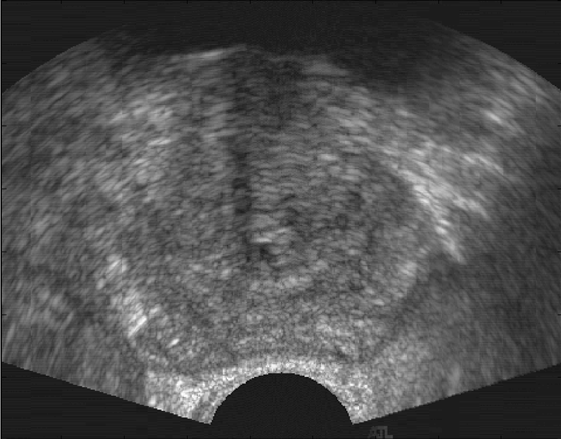
\includegraphics[width=0.45\columnwidth]{P069_US_Intensity}}\hfill
	\subfloat[][GMM-FEM\label{fig:exp1gmmfem}]{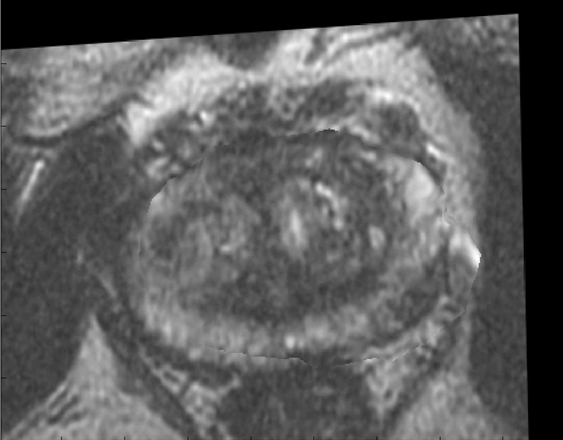
\includegraphics[width=0.45\columnwidth]{P069_MR_FEM_Intensity}}\\
	\subfloat[][Magnitude of the deformation field (mm)\label{fig:exp1def}]{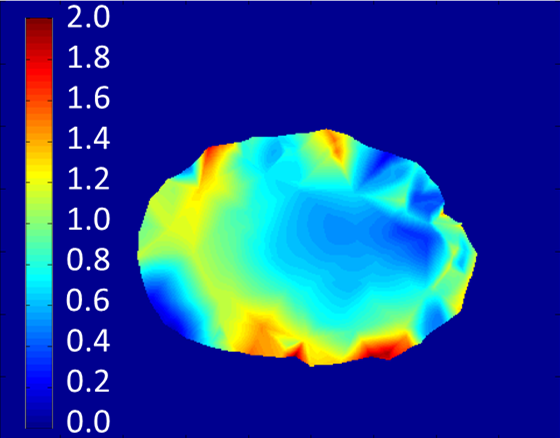
\includegraphics[width=0.45\columnwidth]{DeformationGridBiopsy2}}\hfill
	\subfloat[][Comparison of (a) and (c)\label{fig:exp1ch}]{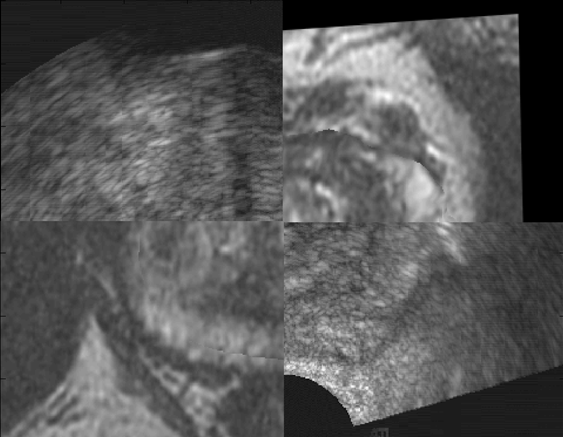
\includegraphics[width=0.45\columnwidth]{P069_CheckerBoard_Intensity}}
    \caption{Typical results for a prostate biopsy data. The axial slice of TRUS (a) and the corresponding GMM-FEM (b) registration results. The deformation map of the nonrigid registration and the corresponding TRUS slice (dashed line) are also shown in (c). The checkerboard of (a) and (b) is shown for comparison. \label{fig:exp1fig2}}
\end{figure}
%%%%%%%%%%%%%%%%%%%%%%%%%%%%%%%%%
\subsubsection{Quantitative Validation}
%%%%%%%%%%%%%%%%%%%%%%%%%%%%%%%%%
Our algorithm was implemented in Matlab (MathWorks, MA), and converges within $\approx10$~seconds on a $3.4$~GHz Intel Core i7 CPU with $8.00$~GB of RAM. To quantify the registration results, we opted to select landmarks on the MR and TRUS images and use these intrinsic fiducials to assess the result of our nonrigid registration. For our ten prostatectomy cases, we selected up to five calcification pairs (a total of thirty) in both modalities per patient, which were validated by a radiologist. For biopsy data, we selected five fiducials per patient consisting of cysts and benign prostatic hyperplasia. This yielded a total of fifty landmarks for validation. Figure~\ref{fig:exp2fiducial1} shows an example of corresponding fiducial pairs in MR and TRUS. The $L_2$ norm of these fiducial pairs were used to quantify the TRE. 

The mean and standard deviation of the TRE and its $p$-value are shown in Tables~\ref{tab:exp2Res1} and \ref{tab:exp1Res1} for prostatectomy and biopsy data, respectively. As seen in Tables~\ref{tab:exp2Res1} and \ref{tab:exp1Res1}, the proposed GMM-FEM registration approach consistently outperforms the TPS-RPM and ICP-FEM methods in terms of TRE. As seen in Table~\ref{tab:exp2Res1} for prostatectomy data, following ICP-FEM and GMM-FEM registration, the mean TRE is improved by $0.2$~mm and $0.5$~mm, respectively. The mean TRE increases for TPS-RPM by $1.0$~mm following TPS-RPM registration. Also as seen in Table~\ref{tab:exp1Res1} for biopsy data, following ICP-FEM and GMM-FEM registration, the mean TRE improves by $0.9$~mm and $1.8$~mm, respectively. The mean TRE increases for TPS-RPM by $2.8$~mm following TPS-RPM registration. This result suggests that FE regularizers are more suitable to propagate surface forces inside the prostate compared to the TPS kernel.

In order to investigate the statistical significance of the registration results, we performed a paired t-test on the TRE between affine and nonrigid registration methods, the null hypothesis being that the affine and each nonrigid registration method share a common mean. The paired t-test rejects the null hypothesis at the 95\% significance level. Thus, the improvement in TRE is shown to be statistically significant.  The p-values are reported in Tables~\ref{tab:exp2Res1} and~\ref{tab:exp1Res1}, for prostatectomy and biopsy data, respectively. 

Finally, in order to investigate the statistical significance of the proposed registration algorithm over other nonrigid registration used for comparison, we performed two  additional paired t-tests. The null hypothesis for the first additional t-test is that the TRE for GMM-FEM and TPS-RPM registration share a common mean. The paired t-test rejects this null hypothesis for both prostatectomy and biopsy data at the 95\% significant level ($p\leq1e-9$). The null hypothesis for the second paired t-test is that the TRE for GMM-FEM and ICP-FEM registration share a common mean. The paired t-test fails to reject the null hypothesis for prostatectomy data at the 95\% confidence. This implies that the improvement of GMM-FEM based registration over ICP-FEM is not significant for full surfaces. However, for biopsy data, the paired t-test rejects the null hypothesis that the TRE for GMM-FEM and ICP-FEM registration share a common mean. This result suggests that the GMM-FEM registration significantly outperforms ICP-FEM for partial surfaces.  \comment{<-- a lot of ``common-mean'' talk.  I'm not sure if this is important.  We may only need to say that the t-test shows it is significant for partial surfaces, but not for full.  Why are they partial here though?  Aren't we using the full US surfaces, and only removing data in the next section?}

%%%%%%%%%%%%%%%%%%%%%%%%%%%%%%%%%
\subsection{Regularization vs. Interpolation}\label{sec:exp2}
%%%%%%%%%%%%%%%%%%%%%%%%%%%%%%%%%
In the second set of experiments, we investigate the robustness of our method when parts of the observations were missing. Robustness is defined as the performance of an algorithm in the presence of disruptive factors~\cite{Jannin02a}. To this end, we removed 10\%, 20\% and 40\% of observation points from base and apex (split equally) and then applied our algorithm to the modified surfaces. In order to quantify the performance, we compared the internal deformation fields with and without missing observations. We explicitly define robustness as the $L_2$ distance of the deformation field with missing observations to the deformation field when no observations are removed. This implicitly defines robustness as the fidelity of the registration in recovering the same deformation field without missing data, i.e. a smaller value corresponds to a better robustness. The results of this experiment are shown in Figure~\ref{fig:exp3reg1} for a typical prostatectomy patient. To highlight the significance of including the FE-based regularization in-loop, we compare to another standard approach: apply a surface-to-surface registration first to estimate surface-to-surface correspondences, then use an FE model in a post-processing step to recover volumetric deformations. For the surface-to-surface registration, we use non-rigid CPD~\cite{Myronenko10a}.  Robustness of the resulting deformation fields are shown in Figure~\ref{fig:exp3reg1} and ~\ref{fig:exp3reg2} from GMM-FEM registration and CPD with post-processing interpolation, respectively.

Excluding outliers in Figures~\ref{fig:exp3reg1}, internal deformations stay below $2.5$~mm when $20\%$ of the observations are removed from the GMM-FEM registration. Compared to Figure~\ref{fig:exp3reg2}, using surface displacements found through CPD as boundary conditions for the FEM yields an larger errors in recovering the deformations when the same number of observations are removed.

As shown in Figure~\ref{fig:exp3hist1}, the robustness of GMM-FEM registration progressively declines as more observations in the base and apex regions are removed. For CPD with post-processing interpolation, as shown in Figure~\ref{fig:exp3hist2}, the robustness of the registration around the surface deteriorates, and surface-bending artifacts appear. Without the volumetric constraints provided by a FE model, points on the surface are not constrained by the interior of the prostate, so have more freedom. As a result, the internal deformation field for CPD found through post-registration interpolation is more sensitive to missing observations. In other words, CPD ignores internal deformation, whereas FEM explicitly minimizes the internal strain energy, providing more of a constraint to resist unnatural changes in shape.
%%%%%%%%%%%%%%%%%%%%%%%%%%%%%%%%%
\begin{figure*}
	\centering
	\subfloat[][GMM-FEM\label{fig:exp3reg1}]{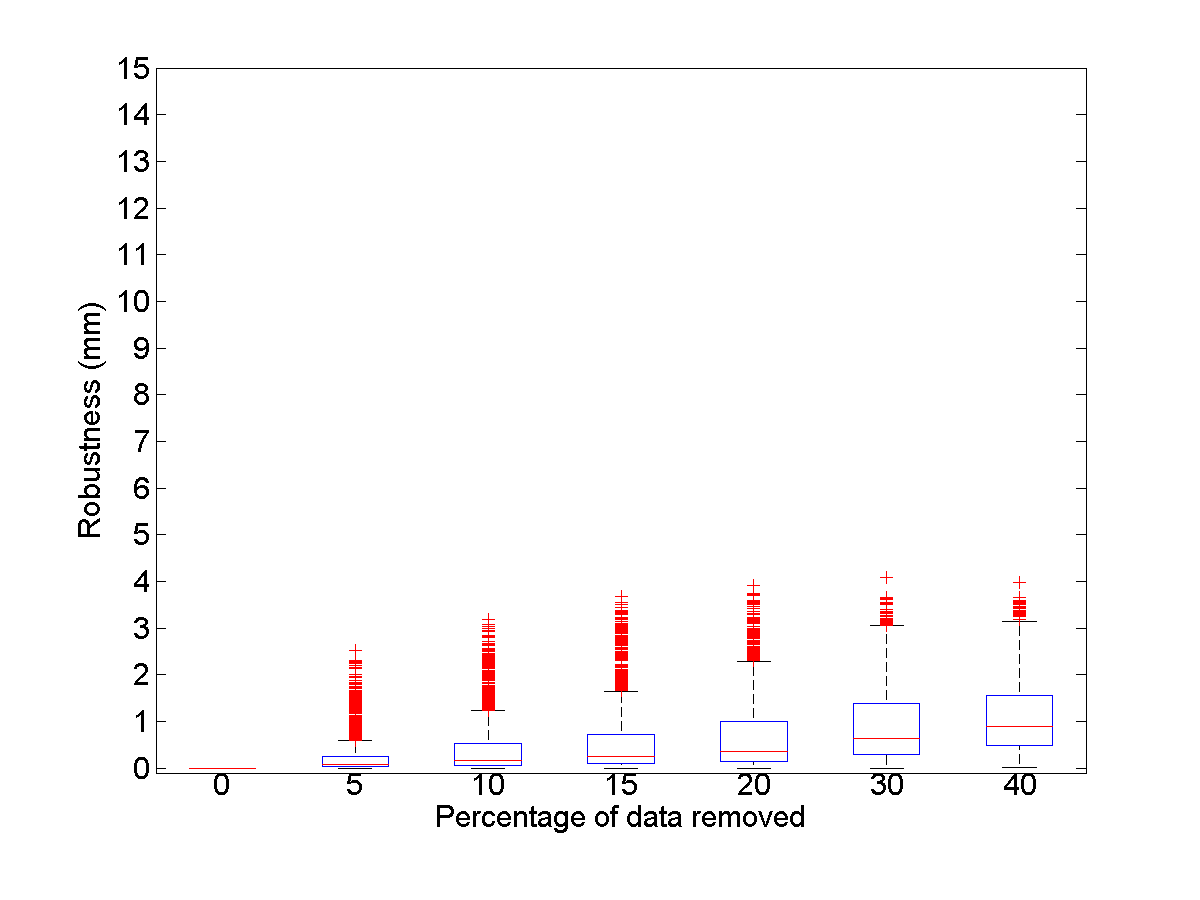
\includegraphics[width=0.49\textwidth]{Boxplot_GMM_FEM}}
	\subfloat[][CPD\label{fig:exp3reg2}]{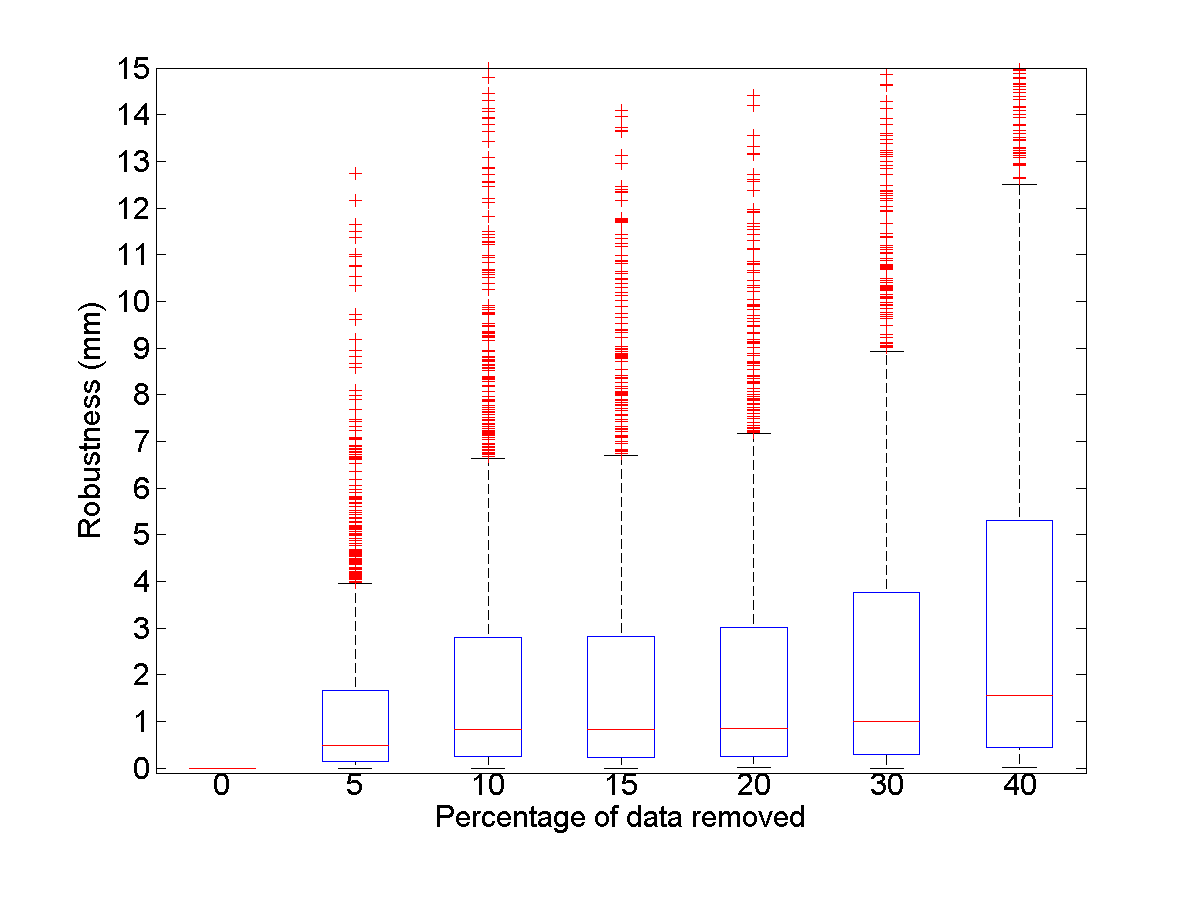
\includegraphics[width=0.49\textwidth]{Boxplot_CPD_FEM}}\\
	\subfloat[][Left to right: Spatial distribution of robustness for GMM-FEM registration when 10\%, 20\% and 40\% of observations are removed.\label{fig:exp3hist1}]{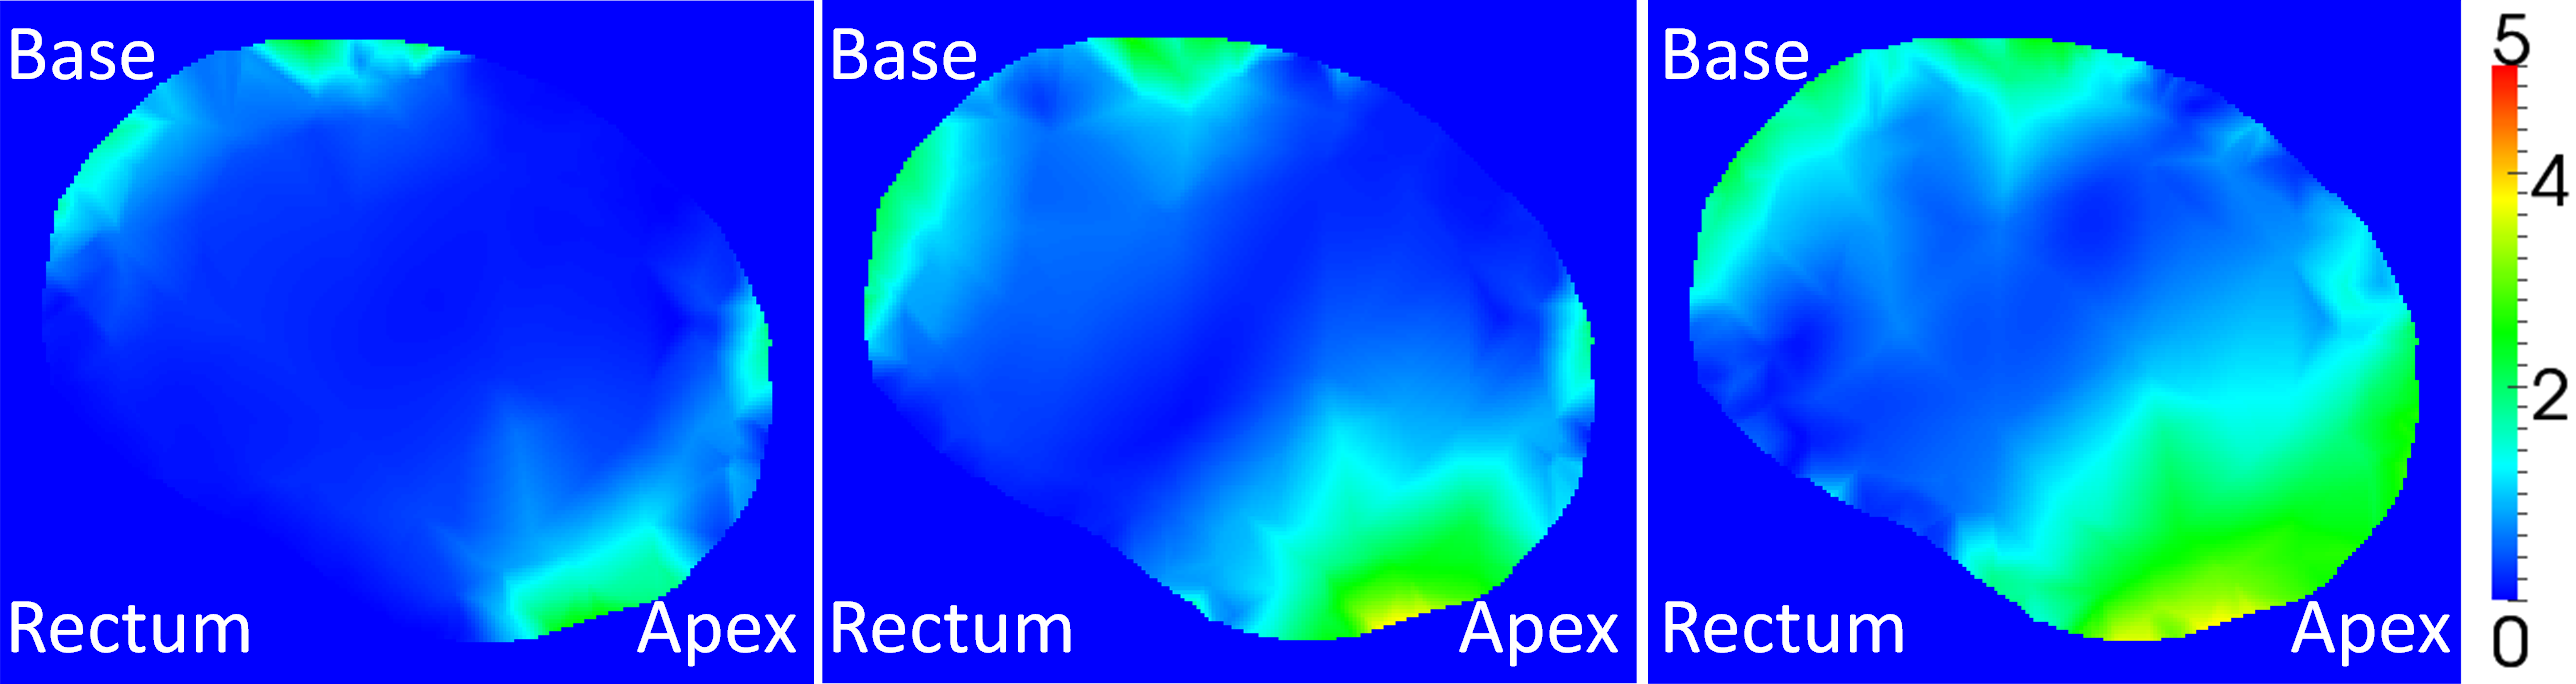
\includegraphics[width=0.49\textwidth]{Spatial_Robustness_GMM_FEM}}\hfill
	\subfloat[][Left to right: Spatial distribution of robustness for CPD registration when 10\%, 20\% and 40\% of data are removed.\label{fig:exp3hist2}]{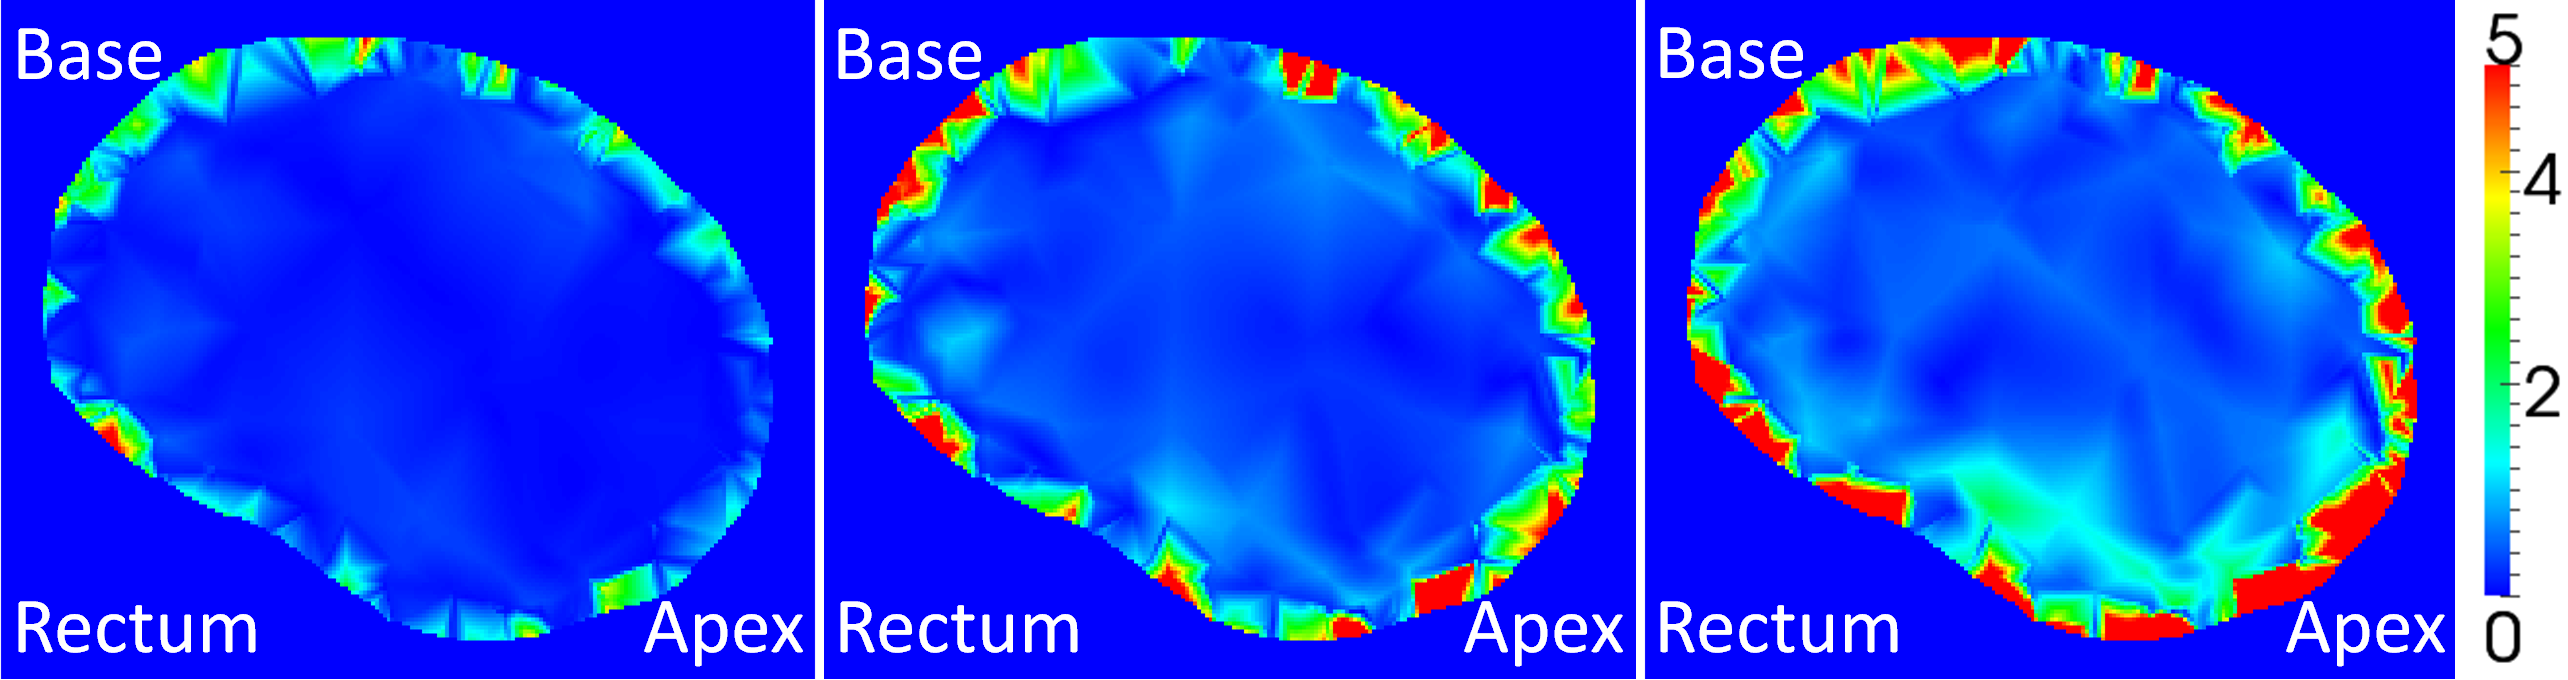
\includegraphics[width=0.49\textwidth]{Spatial_Robustness_CPD}}
    \caption{Comparison of in-loop regularization (a) and post-registration interpolation (b) when $w$ percent of the data is removed with $E=5.0$~kPa and $\nu=0.49$. Sagittal slice of robustness for GMM-FEM (c) and CPD (d) registration when different amounts of observations are removed. For better visualization, distances larger than 5~mm are shown in the same color. \label{fig:exp3fig1}}
\end{figure*}
%%%%%%%%%%%%%%%%%%%%%%%%%%%%%%%%%
\subsection{Sensitivity to Biomechanical Parameters}\label{sec:exp3}
%%%%%%%%%%%%%%%%%%%%%%%%%%%%%%%%%
In the final set of experiments, we investigate robustness of our method to changes in regularization weight, Young's modulus and Poisson's ratio. Under the assumption of homogeneous elasticity, it can be shown that the stiffness matrix has a linear relationship with the Young's modulus (see Equations~\eqref{eq:material} and \eqref{eq:stiffness}). As a result, our registration only has two free biomechanical parameters: 1) the product of the regularization weight and elasticity; and 2) Poisson's ratio. In order to examine the sensitivity of our registration method to these parameters, we perturbed the regularization weight and Poisson's ratio for one of our prostatectomy patients. Figure~\ref{fig:exp4fig1} shows the robustness of our registration method for different regularization weights and Poisson's ratios.

As seen in Figure~\ref{fig:exp4weight}, the GMM-FEM registration can be sensitive to the regularization weight. When tuning this parameter, the registration approach exhibited three distinct behaviors. For large regularization weights, in this case $\beta\geq1.0$, the FEM behaved similar to a rigid object. For very small regularization weights, in this case $\beta\leq0.05$, the FEM does not provide any regularization and the surface is allowed to move independently of interior nodes. Finally, for regularization values in between two extremes, the registration is constrained using the biomechanical properties of the tissue.  This parameter should be tuned to trade-off between surface-fitting and internal deformation. Figure~\ref{fig:exp4hist1} shows the spatial distribution of robustness for three different behaviors described above. The deformation field at the center of the prostate seems more robust to perturbations in the regularization weight compared to the surface. This most likely is due to the fact that the nodes in this region are further away from the surface of the prostate, and as a result, surface forces and biomechanical deformations do not have a large effect in this region.

Figure~\ref{fig:exp4Poisson} shows the sensitivity of the internal deformation field to Poisson's ratio. Apart from the numerical instability of Poisson's ratio near $0.5$, the registration seems less sensitive to perturbations in this parameter compared to the regularization weight. As seen in Figure~\ref{fig:exp4hist2}, similar to changes in regularization weight, perturbations in Poisson's ratio seem to affect the composition of the deformation field near the boundary more than interior regions.
%%%%%%%%%%%%%%%%%%%%%%%%%%%%%%%%%
\section{Discussion and Conclusions}\label{sec:disc}
%%%%%%%%%%%%%%%%%%%%%%%%%%%%%%%%%
In this paper, we presented a novel nonrigid surface-based registration approach that is robust to missing data. The proposed registration algorithm converges within ten seconds on a regular desktop PC. We showed the internal deformation found through our proposed method to be robust up to $2.5$~mm when 20\% of observations are removed. This in-loop regularization was approximately 2.5$\times$ more robust compared to post-registration interpolation of the internal deformation field.  A nice advantage of the algorithm is that it estimates point-correspondences and optimal node displacements in a single minimization step, which is in contrast to all other FE-based approaches.  This is one of the contributing factors to the efficiency of the algorithm.  We also obtain a full volumetric deformation field for the object of interest as a by-product of the regularization, whereas in many existing surface-based approaches, volumetric deformation needs to be estimated with an additional post-processing step.

The GMM-FEM registration method employs probabilistic assignment to establish correspondences and uses a uniform distribution to reject false correspondences for outliers and missing data. While this property is useful for our registration problem, the algorithm rejects large deformations as outliers when the estimate of missing data is set to a large value. One possible extension of this work could be to decouple the effects of missing data and outliers when soft correspondences are made.

One shortcoming of our algorithm is that it requires the MR and TRUS to be segmented prior to the registration. While the MR can be segmented days ahead of time, the 3D-TRUS needs to be segmented within minutes due to clinical requirements. One possible solution is to use an existing fast segmentation method~\cite{Qiu12a}. Of course, since the method is designed to be extremely robust to missing data, we suggest to only segment regions in which the boundary of the anatomy can be clearly distinguished, such as in the mid-gland. This can also help speed up the segmentation process.

In Section~\ref{sec:exp1} we investigated the performance of our registration method using fiducial pairs found in the interior of the prostate. The GMM-FEM algorithm yields a statistically significant improvement over affine ($0.5$~mm) and rigid ($1.8$~mm) registration. While the improvement is small, it should be compared to the acceptable error bounds of a targeted biopsy system. With a TRE of $2.5$~mm, one can obtain a confidence interval corresponding to two standard deviations from the mean, i.e. the estimated true center of the tumor. If this requirement is met, then 95\% of registered targets come within the clinically significant $5$~mm radius~\cite{Karnik10a}. Our improvement on TRE brings us closer to the acceptable error bounds of a targeted biopsy system.

In this paper, we used a linear, homogeneous material to create the prostate FEM. However for most soft tissue, some degree viscoleastic, poroelastic, anisotropic and nonlinear response is expected when a mechanical force is applied. If the nonlinear response is significant, non-linear models, such as Mooney-Rivlin, can easily be included by linearizing about the current deformation state and updating the stiffness matrix at each iteration. This will introduce an additional synthetic force to be added to the objective function that encodes the current state.  As for the tissue elastic modulus, the registration is most sensitive to the estimate of the Young's modulus of the prostate. Currently, elastography is not part of a prostate biopsy protocol. However, if additional information about the elastic properties of the tissue is available, this information can be added into our framework through the stiffness matrix, allowing for non-uniform stiffness, which could potentially improve the registration results.
%%%%%%%%%%%%%%%%%%%%%%%%%%%%%%%%%
\begin{figure*}
	\centering
	\subfloat[][Regularization weight\label{fig:exp4weight}]{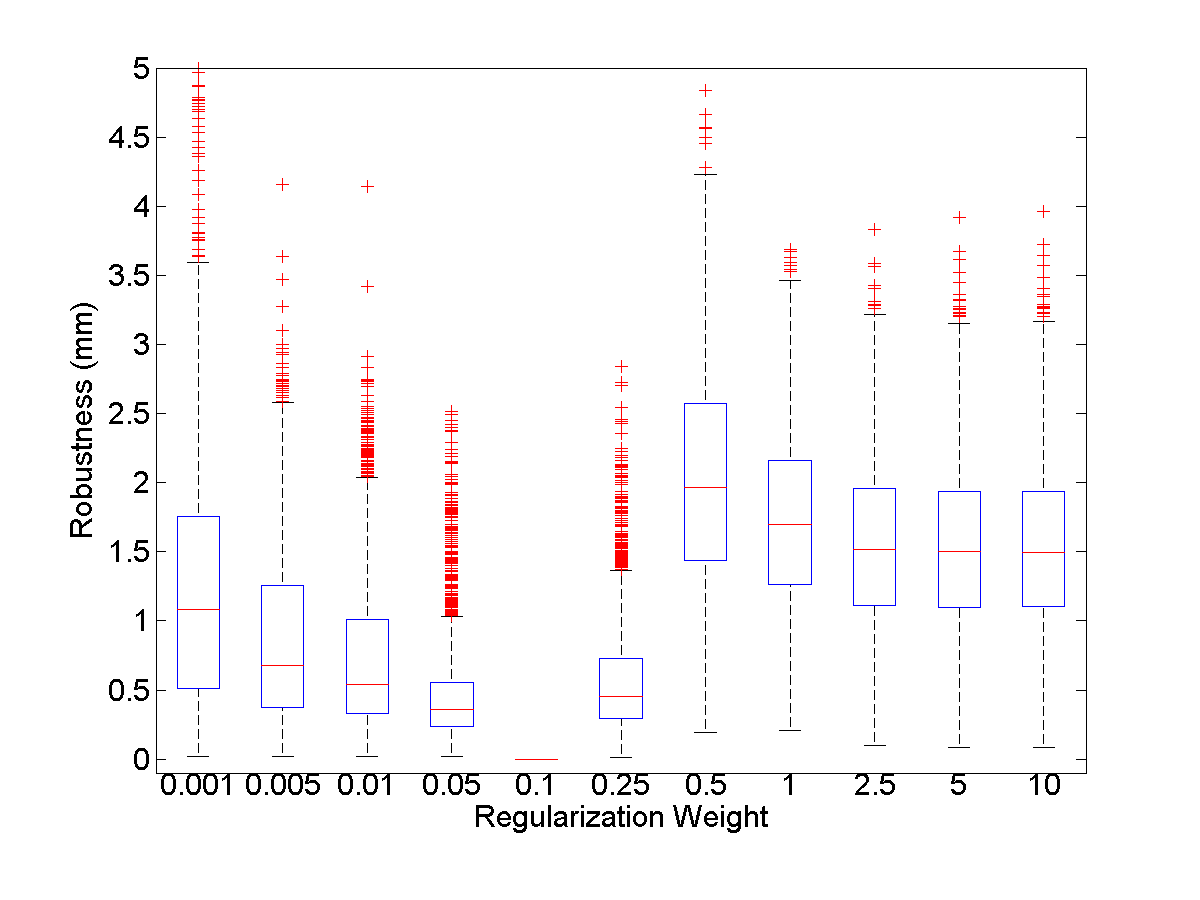
\includegraphics[width=0.49\textwidth]{EffectOfRegularization}}
	\subfloat[][Poisson's ratio\label{fig:exp4Poisson}]{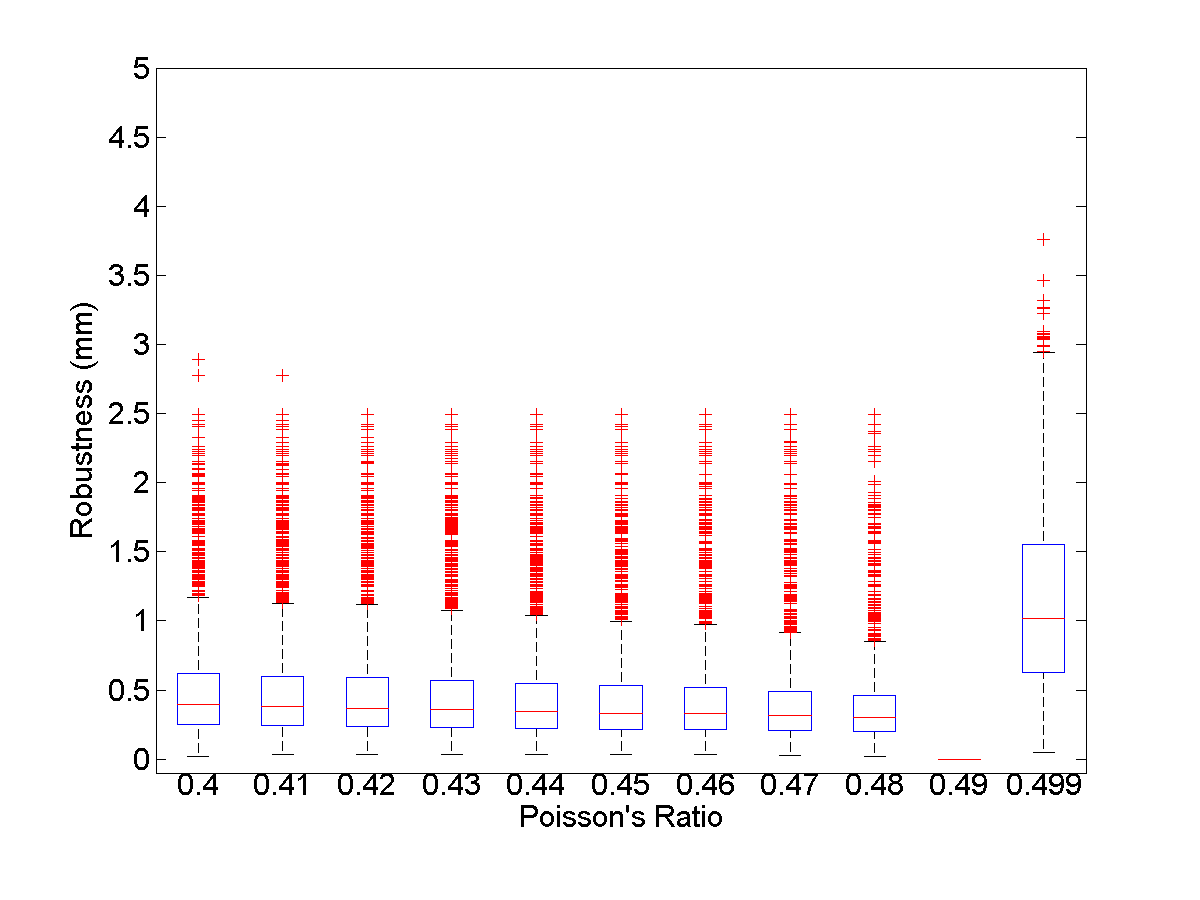
\includegraphics[width=0.49\textwidth]{EffectOfPoisson}}\\
	\subfloat[][Left to right: Spatial distribution of robustness when regularization weight is changed to 0.05, 0.5 and 1.0, respectively.\label{fig:exp4hist1}]{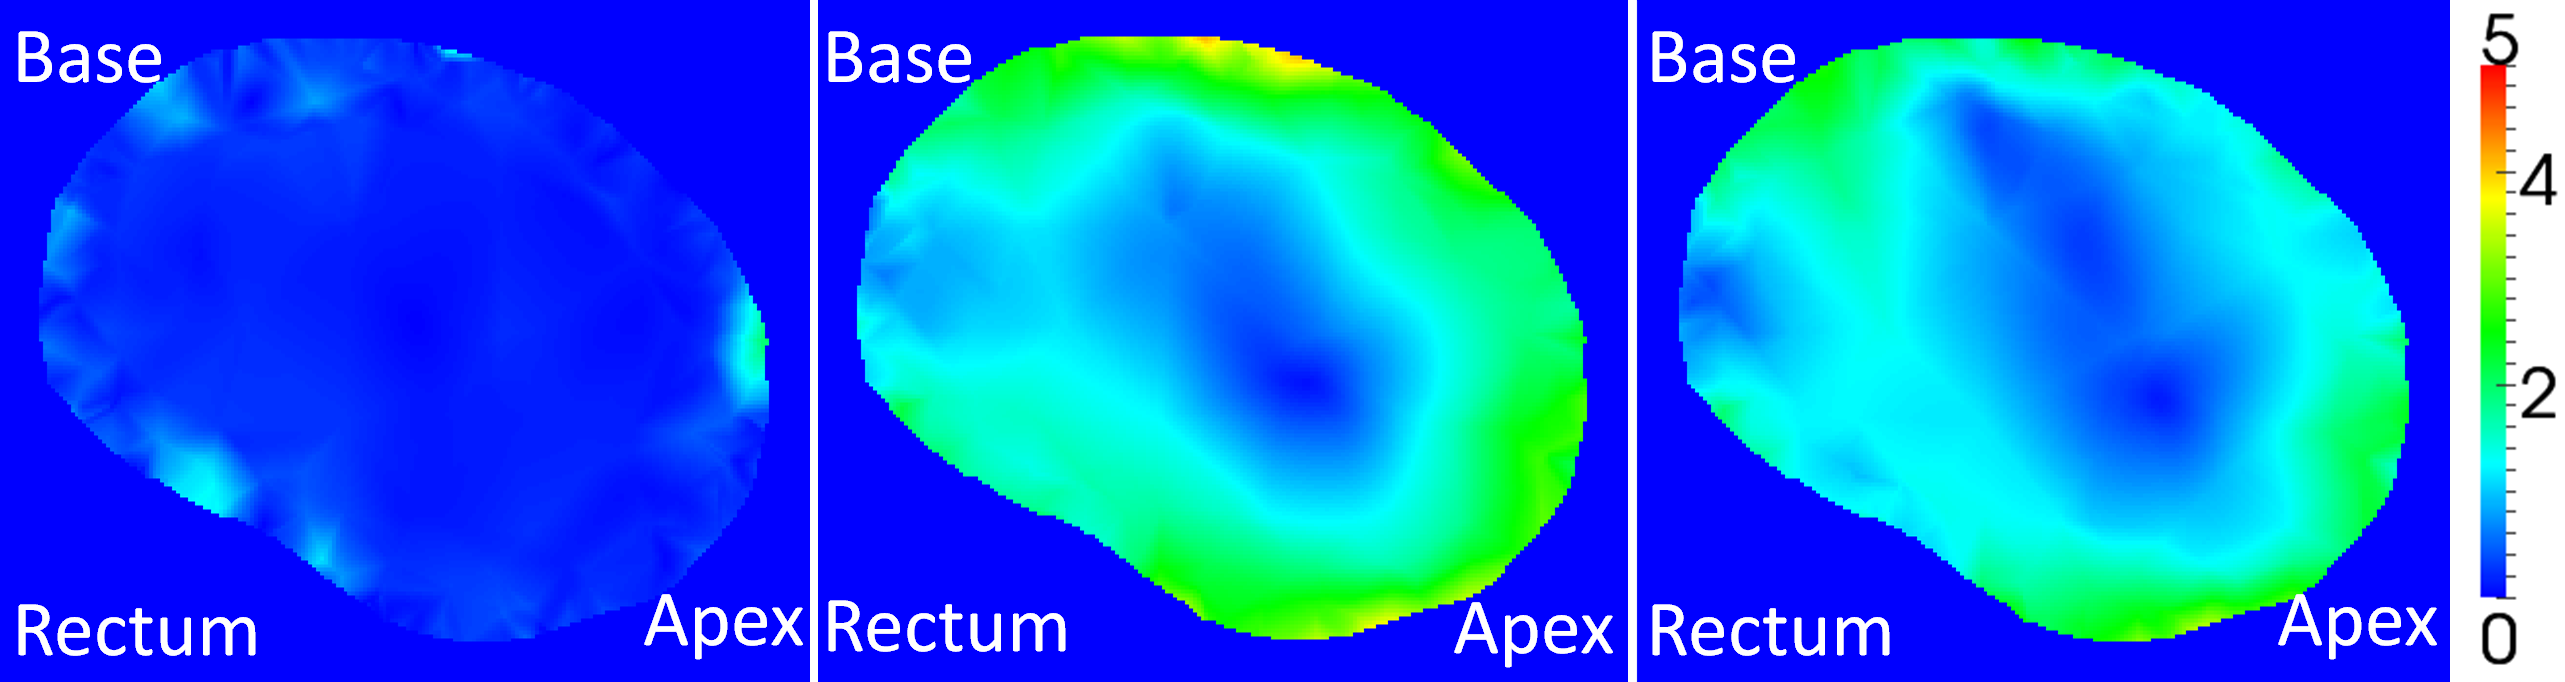
\includegraphics[width=0.49\textwidth]{RobustnessWeight}}\hfill
	\subfloat[][Left to right: Spatial distribution of robustness when Poisson's ratio is changed to 0.40, 0.45 and 0.499, respectively.\label{fig:exp4hist2}]{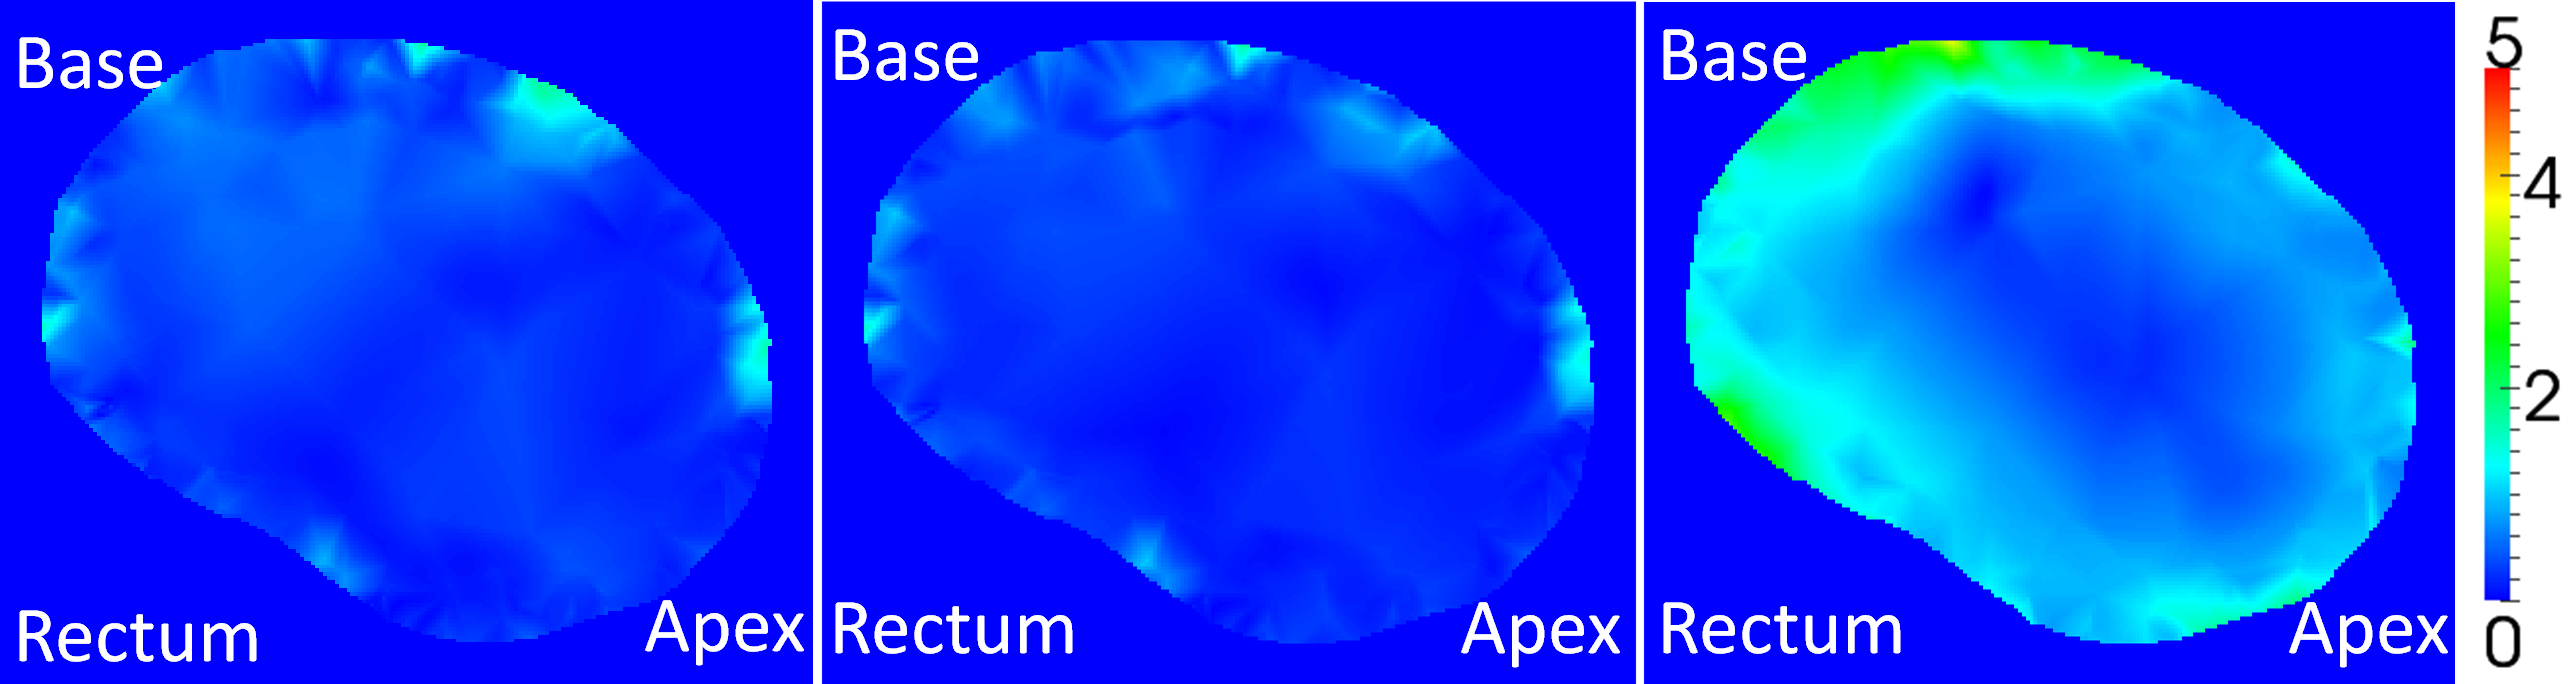
\includegraphics[width=0.49\textwidth]{Robustness_PoissonRatio}}
    \caption{Robustness of GMM-FEM registration for different regularization weights (a) and Poisson's ratios (b). Biomechanical parameters are perturbed around parameters which provided the best surface overlap ($E=5.0$~kPa, $\nu=0.49$ and $\beta=0.1$). For better visualization, distances larger than 5~mm are shown with the same color. \label{fig:exp4fig1}}
\end{figure*}
%%%%%%%%%%%%%%%%%%%%%%%%%%%%%%%%%
\appendices
%%%%%%%%%%%%%%%%%%%%%%%%%%%%%%%%%
\section{}\label{ap:FEM}
%%%%%%%%%%%%%%%%%%%%%%%%%%%%%%%%%
For a static FEM that encapsulates a region $\Omega$, the stiffness matrix is derived by minimizing the total energy of the model:
%%%%%%%%%%%%%%%%%%%%%%%%%%%%%%%%%
\begin{equation} \label{eq:FEMst}
  E(\Omega) = \int_\Omega W(x)dx
\end{equation}
%%%%%%%%%%%%%%%%%%%%%%%%%%%%%%%%%
where $W=\sigma^T\epsilon$ is the elastic energy of a linear material. $\sigma$, $\epsilon$ represents the stress and strain, respectively. If external body forces, $f(.)$ and Dirichlet boundary conditions, $b(.)$, are present, additional terms are added to Equation~\eqref{eq:FEMst}
%%%%%%%%%%%%%%%%%%%%%%%%%%%%%%%%%
\begin{eqnarray} \label{eq:FEMen}
  E(\Omega) = \int_\Omega \sigma^T(x)\epsilon(x) dx + \int_\Omega u^T(x)f(x)dx\nonumber\\
  \text{subject to } \left.u(x)\right|_{\partial \Omega} = b(x),
\end{eqnarray}
%%%%%%%%%%%%%%%%%%%%%%%%%%%%%%%%%
where $u(.)$ is the displacement over the volume. In finite element analysis (FEA), displacements are discretized over the volume as
%%%%%%%%%%%%%%%%%%%%%%%%%%%%%%%%%
\begin{equation} \label{eq:FEMdisc}
  u(x) = \sum_{i=0}^N\phi_i(x)u_i
\end{equation}
%%%%%%%%%%%%%%%%%%%%%%%%%%%%%%%%%
where the shape functions $\{\phi_i\}$ form a partition over the space
%%%%%%%%%%%%%%%%%%%%%%%%%%%%%%%%%
\begin{align}
 \sum_{i=0}^N\phi_i(x) = 1, \quad \forall x\in\Omega.
\end{align}
%%%%%%%%%%%%%%%%%%%%%%%%%%%%%%%%%
The set $\{u_i\}$ describes the degrees of freedom for the given FEM. Each distinct region where a set of the shape functions overlap is called an element. Furthermore, the shape functions are typically defined at a set of points $\{x_i\}$ such that
%%%%%%%%%%%%%%%%%%%%%%%%%%%%%%%%%
\begin{align}
  \phi_k(x_j)& =  \begin{cases}
		    1, & j=k\\
		    0, & j\neq k
		  \end{cases}.
\end{align}
%%%%%%%%%%%%%%%%%%%%%%%%%%%%%%%%%
These $\{x_i\}$ points are referred to as nodes. In such a case, we have $u(x_i)=u_i$ and $\{u_i\}$ are the displacements at the nodes. Substituting equation \eqref{eq:FEMdisc} into an expression for strain, we can write
%%%%%%%%%%%%%%%%%%%%%%%%%%%%%%%%%
\begin{align}
  \epsilon(x) & = \sum_{i=1}^N B_i(x) u_i,\\
  B_i & = \begin{bmatrix}
	  \di{\phi_i}{x_1} & 0 & 0\\
	  0 & \di{\phi_i}{x_2} & 0\\
	  0 & 0 & \di{\phi_i}{x_3}\\
	  \di{\phi_i}{x_2} & \di{\phi_i}{x_1} & 0\\
	  \di{\phi_i}{x_3} & 0 & \di{\phi_i}{x_1}\\
	  0 & \di{\phi_i}{x_3} & \di{\phi_i}{x_2}
        \end{bmatrix}
\end{align}
%%%%%%%%%%%%%%%%%%%%%%%%%%%%%%%%%
For a linear FEM, the stress-strain relationship is written as
%%%%%%%%%%%%%%%%%%%%%%%%%%%%%%%%%
\begin{align}
  \sigma(x) & = D\epsilon(x),\\
  D & = \begin{bmatrix}
	  \lambda +2\mu & \lambda & \lambda  & 0 & 0 & 0\\
	  \lambda &  \lambda +2\mu & \lambda & 0 & 0 & 0\\
	  \lambda & \lambda & \lambda +2\mu & 0 & 0 & 0\\
	  0 & 0 & 0 & \mu & 0 & 0\\
	  0 & 0 & 0 & 0 & \mu & 0\\
	  0 & 0 & 0 & 0 & 0 & \mu
        \end{bmatrix}\label{eq:material}\\
  \lambda & = \dfrac{E\nu}{(1+\nu)(1-2\nu)} \notag\\
  \mu & = \dfrac{E}{2(1+\nu)}, \notag
\end{align}
%%%%%%%%%%%%%%%%%%%%%%%%%%%%%%%%%
where $E$ is the Young's Modulus, and $\nu$ is Poisson's ratio. Substituting all these expressions into Equation~\eqref{eq:FEMen}, we arrive at the system:
%%%%%%%%%%%%%%%%%%%%%%%%%%%%%%%%%
\begin{align} \label{eq:discreteenergy}
   E(\Omega) & = \sum_{i=1}^N\sum_{j=1}^N u_j^T \left[\int_\Omega B_j^TDB_i dx\right]\, u_i \notag\\
   &+ \int_\Omega \phi_i(x)f^T(x) dx\,u_i.
\end{align}
%%%%%%%%%%%%%%%%%%%%%%%%%%%%%%%%%
These integrals are in terms of the absolute coordinate system, and, as a result, describe the deformed state of the object. In general, expressions for the deformed shape functions, $\phi_i$, are not available. Therefor, it is common practice to do a change of variables so integration can be performed over the rest shape. This introduces a Jacobian, $\di{x}{X}$, into Equation~\eqref{eq:discreteenergy} such that
%%%%%%%%%%%%%%%%%%%%%%%%%%%%%%%%%
\begin{align}
  E(\Omega) & = \sum_{i=1}^N\sum_{j=1}^N u_j^T \left[\int_{\Omega_0} B_j^TDB_i \left|\di{x}{X}\right| dX\right]\, u_i \notag\\
  & + \int_{\Omega_0} \phi_i(X)f(X) \left|\di{x}{X}\right|dX\,u_i.
  \label{eq:strainenergy}
\end{align}
%%%%%%%%%%%%%%%%%%%%%%%%%%%%%%%%%
This yields the following stiffness matrix when the elastic energy is minimized
%%%%%%%%%%%%%%%%%%%%%%%%%%%%%%%%%
\begin{align}
 K_{i,j} & = \left[\int_{\Omega_0} B_j^TDB_i \left|\di{x}{X}\right| dX\right], \label{eq:stiffness}
\end{align}
%%%%%%%%%%%%%%%%%%%%%%%%%%%%%%%%%
which depends on the current deformed state due to the Jacobian term. Thus, the stiffness matrix evolves over time in a dynamic simulation. Under the assumption of small deformations, the approximation of $\left|\di{x}{X}\right|\approx I$ would yield a fixed stiffness matrix. For a more in-depth discussion, see~\cite{Bonet00a}.
%%%%%%%%%%%%%%%%%%%%%%%%%%%%%%%%%
\ifCLASSOPTIONcaptionsoff
  \newpage
\fi

\bibliography{tmi}
\bibliographystyle{plain}

\end{document}